\documentclass[letterpaper,12pt,fleqn]{article}
%\VignetteIndexEntry{Introduction to PBStools}
%\VignettePackage{PBStools}

% Packages
%\usepackage{Sweave}
\usepackage{graphicx}
\usepackage{verbatim,fancyvrb}
\usepackage[top=1in, bottom=1in, left=1in, right=1in]{geometry} %  page margins
\usepackage[font=small,format=plain,labelfont=bf,indention=0.25in,labelsep=period,justification=raggedright]{caption}
%\usepackage[font=small,format=plain,labelfont=bf,up,textfont=it,up]{caption}
\usepackage{parskip}

\usepackage[hyphens]{url}
\def\UrlFont{\small\tt}

\usepackage[round]{natbib}
\usepackage{lscape}
\usepackage[utf8]{inputenc}
\usepackage{mathtools}
\usepackage[multiple]{footmisc}
\usepackage{longtable,array} % need array when specifying a ragged right column:  >{\raggedright\arraybackslash}{p2in}
\usepackage{xifthen}         % provides \ifthenelse and \isempty
%\usepackage{amsmath}
  \setlength{\mathindent}{0.5in}
%\usepackage{framed}
%\usepackage{float}
%\usepackage{fancyhdr}

\usepackage{hyperref}
%\usepackage[bookmarks,bookmarksdepth=3]{hyperref}

% from Sweave.Rnw in C:\Apps\R\R300\library\utils\doc
\hypersetup{%
colorlinks,%
plainpages=true,%
linkcolor=black,%
citecolor=black,%
urlcolor=blue,%
%pdfstartview=FitH,% or Fit
pdfstartview=Fit, %{XYZ null null 1},%
pdfview={XYZ null null null},%
pdfpagemode=UseOutlines,% for bookmarks
pdfauthor={Rowan Haigh and Jon T. Schnute},%
pdftitle={PBStools User's Guide},%
pdfsubject={Software for semi-serious scientists}%
}

\raggedright
%\setlength{\hangindent}{0.25in}
\def\noi{\noindent}
\def\noh{\noindent \hangindent=\parindent}
\def\tab{\hspace{0.5 in}}
\newcommand\tstrut{\rule{0pt}{2.4ex}}         % top strut for table row
\newcommand\bstrut{\rule[-1.0ex]{0pt}{0pt}}   % bottom strut for table row

% For colors
\usepackage{color}
\definecolor{red}{rgb}{0.8039216,0.2156863,0}
\definecolor{green}{rgb}{0, 1, 0}
\definecolor{blue}{rgb}{0, 0, 1}
\definecolor{slategrey}{rgb}{0.4392157, 0.5019608, 0.5647059}
\definecolor{deepskyblue}{rgb}{0, 0.7490196, 1}
\definecolor{gainsboro}{rgb}{0.8627451,0.8627451,0.8627451}
\definecolor{aliceblue}{RGB}{240, 248, 255}
\definecolor{dodgerblue}{RGB}{24, 116, 205}
\definecolor{moccasin}{RGB}{255, 236, 204}
\definecolor{honeydew}{RGB}{240, 255, 240}

% Definitions
%\newfont{inc}{inconsolata} 
\newcommand{\slan}{{\tt S}}
\newcommand{\rlan}{{\tt R}}
\newcommand{\pbsd}{{\tt PBSdata}}
\newcommand{\pbsf}{{\tt PBSfishery}}
\newcommand{\pbst}{{\tt PBStools}}
\newcommand{\pbsdat}{{\it PBS Data}}
\newcommand{\tcl}{{\tt Tcl/Tk}}

% from RODBC.Rnw
\newcommand{\code}[1]{\small\texttt{#1}\normalsize}
\newcommand{\pkg}[1]{{\bf #1}}
\newcommand{\var}[1]{\emph{#1}}
\newcommand{\link}[1]{#1}
\newcommand{\sQuote}[1]{`#1'}
\newcommand{\dQuote}[1]{``#1''}
\newcommand{\eqn}[1]{\begin{equation}#1\end{equation}}
%\newcommand{\eqn}[1]{\hspace{0.5in}$#1$}
\newcommand{\gfrac}[2]{\genfrac{}{}{}{0}{#1}{#2}}
%\newcommand{\URL}[1]{\small\url{#1}\normalsize}

\newcommand{\gui}[1]{\small\textmd{\textsf{#1}}\normalsize}
\newcommand{\db}[1]{\small\textmd{\textsf{#1}}\normalsize}
\newcommand{\func}[1]{{\textcolor{dodgerblue} {#1}}}
\newcommand{\ital}[1]{{\it #1}}
\newcommand{\bold}[1]{{\bf #1}}
\newcommand{\under}[1]{{\underline {#1}}}

\newcommand{\red}[1]{{\textcolor{red} {#1}}}
\newcommand{\blue}[1]{{\textcolor{blue} {#1}}}
\newcommand{\grey}[1]{{\textcolor{slategrey} {#1}}}
\newcommand{\sky}[1]{{\textcolor{deepskyblue} {#1}}}
%\newcommand{\dfo}[1]{{\colorbox{aliceblue}{\color{slategrey} {#1}}}}
%\colorbox{declared-color1}{\color{declared-color2}{text}}

\newcommand\pbsfig[4]{    % #1=filename, #2=main caption, #3=figure height, #4=short caption
	\begin{figure}[ht!] %[htbp]
	\centering
	\includegraphics[width=6.5in,height=#3in,keepaspectratio=TRUE]{#1.png}
	% http://xelatex.blogspot.ca/2008/03/newcommand-with-optional-argument.html
	\ifthenelse{\isempty{#4}}
		{\caption[#2]{(\emph{#1}) #2}\vspace{-2ex}}
		{\caption[#4]{(\emph{#1}) #2}\vspace{-2ex}}
	\label{fig:#1}
	\end{figure}
	%\clearpage
}
\newcommand\pbstest[4]{    % #1=filename, #2=main caption, #3=figure height, #4=short caption
	\begin{figure}[ht!] %[htbp]
	\centering
	\includegraphics[width=6.5in,height=#3in,keepaspectratio=TRUE]{#1.png}
	% http://xelatex.blogspot.ca/2008/03/newcommand-with-optional-argument.html
	\ifthenelse{\isempty{#4}}  %{#2}{#4}% 
	{\caption[#2]{(\emph{#1}) #2}\vspace{-2ex}}
	{\caption[#4]{(\emph{#1}) #2}\vspace{-2ex}}
	\label{fig:#1}
	\end{figure}
	%\clearpage
}
\newcommand\pbsfigland[3]{    % filename is #1, text is #2, figure height is #3
	\clearpage
	\begin{figure}[ht] %[htbp]
	\begin{minipage}[c]{4.25in}
	\centering
	\includegraphics[width=4.0in,height=10in,keepaspectratio=TRUE]{#1.png}
	\end{minipage}
	\hspace{0in}
	\begin{minipage}[c]{4.75in}
	\centering
	\includegraphics[width=4.25in,height=10in,keepaspectratio=TRUE]{#2.png}
	\end{minipage}
	\caption{#3}\vspace{-2ex}
	\label{fig:#1}
	\end{figure}
}
\newcommand\example[1]{    % #1 = function name (or any text) for example line.
	\textbf{\emph{Example~(#1):}}\\ \vspace{3 pt}
}
\newcommand\results[1]{    % #1 = function name (or any text) for example line.
	\textbf{\emph{Output~(#1):}}\\ \vspace{3 pt}
}
% Coloured box environment
% Source: Manifold @ http://answers.google.com/answers/threadview?id=282787
\makeatletter\newenvironment{dfobox}{%
   \begin{lrbox}{\@tempboxa}\begin{minipage}{\columnwidth}\raggedright}{\end{minipage}\end{lrbox}%
   \colorbox{moccasin}{\usebox{\@tempboxa}}
}\makeatother

% Example box environment
% Source: Manifold @ http://answers.google.com/answers/threadview?id=282787
\makeatletter\newenvironment{examplebox}{%
   \begin{lrbox}{\@tempboxa}\begin{minipage}{\textwidth}\raggedright}{\end{minipage}\end{lrbox}%
   \colorbox{aliceblue}{\usebox{\@tempboxa}}
}\makeatother

% Output box environment
% Source: Manifold @ http://answers.google.com/answers/threadview?id=282787
\makeatletter\newenvironment{outputbox}{%
   \begin{lrbox}{\@tempboxa}\begin{minipage}{\textwidth}\raggedright}{\end{minipage}\end{lrbox}%
   \colorbox{honeydew}{\usebox{\@tempboxa}}
}\makeatother

% Get rid of all that margin space
\topmargin -0.5in 
\oddsidemargin 0in \evensidemargin 0in
\textheight 9.0in \textwidth 6.5in

% Undoing the dumb defaults for float
% http://mintaka.sdsu.edu/GF/bibliog/latex/floats.html
% Alter some LaTeX defaults for better treatment of figures:
% See p.105 of "TeX Unbound" for suggested values.
% See pp. 199-200 of Lamport's "LaTeX" book for details.
% General parameters, for ALL pages:
  \renewcommand{\topfraction}{0.9}	% max fraction of floats at top
  \renewcommand{\bottomfraction}{0.8}	% max fraction of floats at bottom
% Parameters for TEXT pages (not float pages):
  \setcounter{topnumber}{2}
  \setcounter{bottomnumber}{2}
  \setcounter{totalnumber}{4}     % 2 may work better
  \setcounter{dbltopnumber}{2}    % for 2-column pages
  \renewcommand{\dbltopfraction}{0.9}	% fit big float above 2-col. text
  \renewcommand{\textfraction}{0.07}	% allow minimal text w. figs
% Parameters for FLOAT pages (not text pages):
  \renewcommand{\floatpagefraction}{0.7}	% require fuller float pages
% N.B.: floatpagefraction MUST be less than topfraction !!
  \renewcommand{\dblfloatpagefraction}{0.7}	% require fuller float pages

%Latex: Squeezing the Vertical White Space
%http://www.terminally-incoherent.com/blog/2007/09/19/latex-squeezing-the-vertical-white-space/
\usepackage[compact]{titlesec}
\titlespacing{\section}{0pt}{*0}{*0}
\titlespacing{\subsection}{0pt}{*0}{*0}
\titlespacing{\subsubsection}{0pt}{*0}{*0}

%===========================================================
\begin{document}
\pagenumbering{roman}

\title{PBStools: User's Guide}
\author{Rowan Haigh and Jon T. Schnute}

\maketitle
\tableofcontents
\listoftables % (lot)
\listoffigures % (lof)
%\clearpage
%\fancyfoot[R]{\small \date{}}

\clearpage
\begin{minipage}{\textwidth}
\vspace*{4in}
\begin{center}
\LARGE\it\grey{Page left blank for printing purposes.}
\end{center}
\vfill % equivalent to \vspace{\fill}
\end{minipage}

%\vspace{4.0 in}
%\centerline{\large\it\grey{Page left blank for printing purposes.}\normalsize}
%-------------------------------------------------
\newpage
\pagenumbering{arabic}

\phantomsection
\addcontentsline{toc}{section}{What is PBStools?} % Adds to bookmarks only
\section* {What is PBStools?}
%\addcontentsline{toc}{section}{\protect\numberline{}What is PBStools?}

\tab \pkg{PBStools} provides an R interface for algorithms commonly used in fisheries. The scope of this package is by no means comprehensive, having grown from the need to satisfy tasks specific to British Columbia (BC) ocean fisheries. Many of the functions provide a quick way to visualize data, and in some cases perform preliminary analyses. Though oriented to users at the Pacific Biological Station (PBS), these functions may provide a broad utility to users at other locales. The User Guide is organised into sections that loosely classify the functions by theme -- (1)~Utility, (2)~Biology, (3)~Fishery, (4)~Survey, (5)~Spatial, (6)~Temporal, and (7)~Catch Reconstruction. Within each section, the functions are described alphabetically.

\tab \pkg{PBStools} depends heavily on two other R package: \pkg{PBSmapping} \citep{Schnute-etal:2004b,Boers-etal:2004} and \pkg{PBSmodelling} \citep{Schnute-etal:2006}. We use the latter to implement several Graphical User Interfaces (GUIs) that facilitate a few select functions. Most functions, however, are designed for use on the command line or in sourced code. Many of the functions invisibly return auxiliary output in a list object called \code{PBStool}, which is located in the temporary working environment \code{.PBStoolEnv}. Accessor functions called \code{ttget}, \code{ttcall}, and \code{ttprint} enable the user to get, call, and print objects from the \code{.PBStoolEnv} environment, while \code{ttput} puts (writes) obects to \code{.PBStoolEnv}.

\tab Amongst the various functions in the package, we include those that implement some of the models published by the authors. For example, \code{calcSG} estimates parameters for the Schnute growth model \citep{Schnute:1981}, which offers a versatile alternative to the von Bertalanffy growth model (\code{calcVB}). The functions presented in the Survey section make use of the binomial-gamma model \citep{Schnute-Haigh:2003} for characterizing survey strata populations when designing or simulating groundfish trawl surveys. The function \code{runCCA} implements the composition analysis of \citet{Schnute-Haigh:2007} to estimate total mortality $Z$ of rockfish (\emph{Sebastes} spp.) using three combined effects: survival at age ($S_a$), fishery selectivity at age ($\beta_a$), and relative recruitment anomalies ($R_a$). Finally, the function \code{buildCatch} provides an efficient method for reconstructing rockfish catch from 1918 to the present along the BC coast \citep{Haigh-Yamanaka:2011}.

\tab Also available in the package directory \code{./library/PBStools/sql} we provide a number of useful SQL queries for DFO\footnote{Department of Fisheries and Oceans, a.k.a. Fisheries and Oceans Canada} commercial fisheries databases -- \db{PacHarvest} (trawl, 1996--2007), \db{PacHarvHL} (hook and line, 1994--2006), \db{GFCatch} (historical landings, 1954--1995), \db{GFBioSQL} (biological samples, 1946--2012), and \db{GFFOS} (integrated fisheries, 2002--present). To launch SQL queries, \pkg{PBStools} relies on the R package \pkg{RODBC}. If you have access to the DFO network and have privileges to query these databases, the function \code{getData} can send the queries to the remote servers and return a data frame called \code{PBSdat} in the global environment. In the document, we highlight queries for DFO personnel using text with a background shaded \code{moccasin}\footnote{RGBs: moccasin=(255,228,181), aliceblue=(240,248,255), honeydew=(240,255,240)}. (Examples are shaded \code{aliceblue} and console output is shaded \code{honeydew}.) Note that many of these queries might act as useful templates for users outside DFO for similar purposes. Querying databases directly via SQL commands from R usually proves much more efficient than launching Microsoft Access Queries from a front-end database shell.

\tab Originally, \pkg{PBStools} evolved over time (2007--2012) within the R package \pkg{PBSfishery}\footnote{found on Google's Project Hosting site: \url{http://code.google.com/p/pbs-fishery/}}, along with a convenient Graphical User Interface (GUI) tool for interacting with \pkg{PBSmapping} and useful datasets (regional boundaries, key codes, example data). In April 2012, we decided to split \pkg{PBSfishery} into three separate libraries -- \pkg{PBStools}, \pkg{PBSmapx}, and \pkg{PBSdata}  -- for distribution on CRAN.

%-------------------------------------------------
\phantomsection
\addcontentsline{toc}{section}{What is PBS?} % Adds to bookmarks only
\subsection* {What is PBS?}
%\addcontentsline{toc}{subsection}{\protect\numberline{}What is PBS?}

\tab The Pacific Biological Station is the oldest fisheries research centre on Canada's Pacific coast and forms part of a network of nine major scientific facilities operated by Fisheries and Oceans Canada. Located in Nanaimo, British Columbia, the Station is home to scientists, technicians, support staff and ships' crews whose common interests are the coastal waters of British Columbia, the Northeast Pacific Ocean, the Western Arctic and navigable waters east to the Manitoba, Saskatchewan border.

\tab PBS was established in 1908 and is the principal centre for fisheries research on Canada's west coast. There are some 22 structures on the site including a four-story office/wet lab building, specialty storage structures for hazardous chemicals and salt water pumping facilities. PBS maintains a number of workshops for research support. There is a wharf used for loading, unloading, and berthage of research vessels, as well as a small boat dock for inshore research boats. PBS also maintains a library and meeting facilities. Aquatic facilities, primarily used by Aquaculture Science, include ambient temperature and heated salt water and fresh water. 

\tab Research at PBS responds to stock assessment, aquaculture, marine environment, habitat, ocean science, and fish productivity priorities. Some fisheries management activities are also conducted here. 

\begin{figure}[h!]
	\centering
	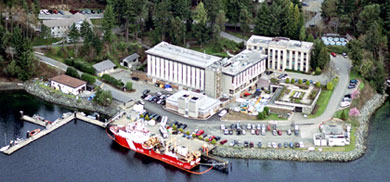
\includegraphics[width=10cm]{PBS.png}
	\quad
	\caption{Pacific Biological Station (PBS), Nanaimo BC}
	\label{fig:PBS}
\end{figure}

For more information, see:\\ \footnotesize
\url{http://www.pac.dfo-mpo.gc.ca/science/facilities-installations/pbs-sbp/index-eng.htm}. \normalsize

\clearpage
%\setcounter{section}{1}
%-------------------------------------------------
\section {Utility functions}

\tab The utility functions described in this section cover a broad range of activities. The number of functions has grown over time and inevitably, some of the functions may replicate the behaviour of functions in other packages. Additionally, the utility of these functions can either decline or cease based on changes in dependent packages. Feedback is appreciated from any users of \pkg{PBStools}.

\subsection {biteData}

\tab Subset a matrix or data frame using a vector object with the same name as one of the fields in the data matrix/frame and return the subset data matrix/frame. If there are no fields with the name of the vector object, the data matrix/frame is returned unaltered.

\tab Due to the current nature of the algorithm, the user cannot supply an ad hoc vector directly as the argument. This means the vector object must exist before calling \code{biteData}.

Not allowed: \code{biteData(swiss,Education=1:5)}\\
Allowed:     \code{Education=1:5; biteData(swiss,Education)}

\begin{examplebox}
\example{biteData}
\begin{Verbatim}[fontsize=\footnotesize]
pbsfun=function(){
  cat("Records in original swiss object by Education\n")
  print(sapply(split(swiss$Education,swiss$Education),length))
  Education=1:5; test=biteData(swiss,Education)
  cat("Records in swiss object subset where Education=1:5\n")
  print(sapply(split(test$Education,test$Education),length))
  invisible() }
pbsfun()
\end{Verbatim}
\end{examplebox}

\begin{outputbox}
\results{biteData}
\begin{Verbatim}[fontsize=\footnotesize]
Records in original swiss object by Education
 1  2  3  5  6  7  8  9 10 11 12 13 15 19 20 28 29 32 53 
 1  3  4  2  4  7  4  3  2  1  5  3  1  1  1  1  2  1  1 
Records in swiss object subset where Education=1:5
1 2 3 5 
1 3 4 2
\end{Verbatim}
\end{outputbox}

\subsection {chewData}

\tab Remove records from a data frame or matrix that contribute little information to unique categories of the factor specified. Records are removed if a specified factor's categories don't number more than the specified minimum. If there are no fields with the name of the specified factor, the data matrix/frame is returned unaltered.

\begin{examplebox}
\example{chewData}
\begin{Verbatim}[fontsize=\footnotesize]
pbsfun=function(){
  cat("Unique records in 'iris$Petal.Width'\n")
  print(sapply(split(iris$Petal.Width,iris$Petal.Width),length))
  test=chewData(iris,"Petal.Width",5)
  cat("'Petal.Width' categories fewer than 5 removed\n")
  print(sapply(split(test$Petal.Width,test$Petal.Width),length))
  invisible() }
pbsfun()
\end{Verbatim}
\end{examplebox}

\begin{outputbox}
\results{chewData}
\begin{Verbatim}[fontsize=\footnotesize]
Unique records in 'iris$Petal.Width'
0.1 0.2 0.3 0.4 0.5 0.6   1 1.1 1.2 1.3 1.4 1.5 1.6 1.7 1.8 1.9   2 2.1 2.2 
  5  29   7   7   1   1   7   3   5  13   8  12   4   2  12   5   6   6   3 
2.3 2.4 2.5 
  8   3   3 
'Petal.Width' categories fewer than 5 removed
0.1 0.2 0.3 0.4   1 1.2 1.3 1.4 1.5 1.8 1.9   2 2.1 2.3 
  5  29   7   7   7   5  13   8  12  12   5   6   6   8
\end{Verbatim}
\end{outputbox}


\subsection {collectFigs}

\tab Collect figures (currently only encapsulated postscript \code{.eps} supported) into one document using a latex compiler (\code{latex.exe}, \code{dvips.exe}, \code{ps2pdf.exe}). The code constructs a \code{.tex} file that uses all available \code{.eps} files in the specified directory. The final result is a bookmarked PDF file called \code{<fout>.pdf}, where \code{fout} is user-supplied prefix for the output file.

\subsection {confODBC}

\tab Use a command line utility found in Windows OS called \code{odbcconf.exe} that configures an ODBC Data Source Name from the system's command line. The function runs the command line utility with the user-supplied information, and configures a User DSN on the his/her computer.

In Windows XP, the new User DSN can be seen by navigating to:\\
\gui{$<$Control Panel$><$Administrative Tools$><$Data Sources (ODBC)$>$} (Figure~\ref{fig:PBStools-confODBC}).

\begin{examplebox}
\example{confODBC}
\begin{Verbatim}[fontsize=\footnotesize]
pbsfun=function(os=.Platform$OS.type,dfo=TRUE) {
  if (os=="windows" && dfo)
    confODBC(dsn="Popsicle", server="GFDB", db="PacHarvest",
      driver="SQL Server", descr="Icy sweet nonsense", trusted=TRUE) 
  else showMessage("Only functional for DFO personnel using Microsoft Windows OS")
  invisible() }
pbsfun()
\end{Verbatim}
\end{examplebox}
%\pbstest{PBStools-confODBC}{ODBC data source configuration for DSN \dQuote{Popsicle}.}{3.25}{Mars attacks}
\pbsfig{PBStools-confODBC}{ODBC data source configuration for DSN \dQuote{Popsicle}.}{3.25}{}

\subsection {convFY}

\tab Convert a vector of dates into a vector of fishing or fiscal years based on a specified month to start the fishing/fiscal year.  The function returns a numeric vector of fishing/fiscal years of equal length to the input vector of dates. The output vector has names representing year-month \code{YYYY-MM}.  If the starting month is set to 1, the output dates also represent calendar years.

\begin{examplebox}
\example{convFY}
\begin{Verbatim}[fontsize=\footnotesize]
pbsfun=function() {
  cat("Fishing years starting in April\n")
  print(convFY(paste("2009-",pad0(1:12,2),"-15",sep="")))
  invisible() }
pbsfun()
\end{Verbatim}
\end{examplebox}

\begin{outputbox}
\results{convFY}
\begin{Verbatim}[fontsize=\footnotesize]
Fishing years starting in April
2009-01 2009-02 2009-03 2009-04 2009-05 2009-06 2009-07 2009-08 2009-09 
   2008    2008    2008    2009    2009    2009    2009    2009    2009 
2009-10 2009-11 2009-12 
   2009    2009    2009
\end{Verbatim}
\end{outputbox}

\subsection {convYM}

\tab Convert a 2-element vector of date limits into a vector of year-months where every month within the limits is represented.  The function returns an expanded character vector of ordered year-months \code{YYYY-MM} between and including the specified date limits. This character vector can be used for labelling and other factor-like routines.

\begin{examplebox}
\example{convYM}
\begin{Verbatim}[fontsize=\footnotesize]
pbsfun=function() {
  cat("Year-month labels between the specified date limits\n")
  print(convYM(c("2009-07-01","2011-11-11")))
  invisible() }
pbsfun()
\end{Verbatim}
\end{examplebox}

\begin{outputbox}
\results{convYM}
\begin{Verbatim}[fontsize=\footnotesize]
Year-month labels between the specified date limits
 [1] "2009-07" "2009-08" "2009-09" "2009-10" "2009-11" "2009-12" "2010-01"
 [8] "2010-02" "2010-03" "2010-04" "2010-05" "2010-06" "2010-07" "2010-08"
[15] "2010-09" "2010-10" "2010-11" "2010-12" "2011-01" "2011-02" "2011-03"
[22] "2011-04" "2011-05" "2011-06" "2011-07" "2011-08" "2011-09" "2011-10"
[29] "2011-11"
\end{Verbatim}
\end{outputbox}

\subsection {convYP}

\tab Convert a vector of dates into one of year-periods through binning the dates into intervals specified in days. The routine actually fudges the integer day interval to a real number that will create even breaks. The function returns a vector (with the same length as the input date vector) that specifies dates as real numbers where the integer part is the year and the fraction part is the proportion of the year corresponding to the bin's right-most value. Each element of the vector also has a name that specifies the year and bin number.

\begin{examplebox}
\example{convYP}
\begin{Verbatim}[fontsize=\footnotesize]
pbsfun=function() {
  x=paste("2009-",c("03-31","06-30","09-30","12-30"),sep="")
  cat("Year periods based on numeric value of input dates\n")
  print(convYP(x,30))
  invisible() };  pbsfun()
\end{Verbatim}
\end{examplebox}

\begin{outputbox}
\results{convYP}
\begin{Verbatim}[fontsize=\footnotesize]
Year periods based on numeric value of input dates
2009-03 2009-06 2009-09 2009-12 
2009.25 2009.50 2009.75 2010.00
\end{Verbatim}
\end{outputbox}

\subsection {createDSN}

\tab Create a suite of User DSNs for PBS groundfish databases, currently hosted on the server \db{SVBCPBSGFIIS}. This function uses \code{confODBC} and will overwrite existing DSNs if they exist. Currently, six DSNs for DFO databases will be created:

\begin{Verbatim}[fontsize=\footnotesize]
GFBioSQL   GFCatch   GFCruise   PacHarvest   PacHarvHL   PacHarvSable
\end{Verbatim}

In XP, the new User DSNs can be seen by navigating to: \\
\gui{$<$Control Panel$><$Administrative Tools$><$Data Sources (ODBC)$>$} (Figure~\ref{fig:PBStools-createDSN}).

\begin{examplebox}
\example{createDSN}
\begin{Verbatim}[fontsize=\footnotesize]
pbsfun=function(os=.Platform$OS.type,dfo=FALSE) {
  if (os=="windows" && dfo) createDSN() 
  else showMessage("Only functional for DFO personnel using Microsoft Windows OS")
  invisible() }
pbsfun()
\end{Verbatim}
\end{examplebox}
\pbsfig{PBStools-createDSN}{ODBC data source configuration for DFO groundfish database DSNs.}{3.25}{}

\subsection {crossTab}

\tab Run a cross tabulation on a data frame, summarizing z-values by specified \sQuote{factors}.
This function requires the R package \pkg{reshape}, and uses the functions \code{melt.data.frame} and \code{cast} therein.
The output reports a cross tabulation of \code{y} with values \code{z} summarized by \code{func}.
The function \code{crossTab} is useful for summarizing data query results (e.g., total catch by year and PMFC major area) when exploring / debugging functions like \code{buildCatch}.

\subsection {fitLogit}

\tab Fit binomial data using a \code{logit} link function in a \code{glm}. The function returns a GLM fit of the binomial data using the specified independent observations. See the \sQuote{Value} section of the \code{glm} help file in the \pkg{stats} package.

\subsection {flagIt}

\tab Take a coordinate \code{(a,b)} and label it using a diagonal line of radius \code{r} and angle \code{A}.
A diagonal dotted line in light grey radiates out from a central coordinate and the coordinate values are used to label the coordinate itself.
The function adjusts for the aspect ratio created by different x- and y-limits, and for different x- and y-dimensions of the plot. 
This ensures that an angle looks correct in the plotting space.
The code invisibly returns a list of the vectors (a,x) and (b,y), the angle in radians, the original x-value calculated in a square Cartesian system, and the final x- and y-coordinates on the periphery of a circle.

\begin{examplebox}
\example{flagIt}
\begin{Verbatim}[fontsize=\footnotesize]
pbsfun = function() {
  plot(0,0,type="n",xlim=c(0,20),ylim=c(0.2,0.8))
  points(10,0.5,pch=20,col="blue")
  for (i in seq(10,360,10))
    flagIt(a=10, b=0.5, r=0.25, A=i,col="blue",cex=0.7)
}; pbsfun()
\end{Verbatim}
\end{examplebox}
\pbsfig{PBStools-flagIt}{The point (10, 0.5) flagged using vectors at 10$^{\circ}$ angles.}{3.0}{}

\subsection {getData}

\tab Attempt to get data from a variety of types (e.g., data objects/files, queries/tables) and remote sources (\code{ORA}, \code{SQL}, \code{MDB}, \code{DBF}, \code{XLS}, \code{FILE}). The data table retrieved is placed in a global data frame object called \code{PBSdat}. If the type is \code{MDB}, the query/table name and the database name are attached as attributes. If the type is \code{SQL} or \code{ORA}, the DB name, query name, and SQL code are attached as attributes. This function, which remains one of the key utilities in \pkg{PBStools} for retrieving data, is essentially a glossy wrapper for the function \code{sqlQuery} in the package \pkg{RODBC}.

\tab There are a few quirks that a user should keep in mind. This function was designed primarily to access remote SQL Server and Oracle databases using files containing structured query language (SQL). Unfortunately, SQL syntax varies between the two database systems but the differences are fewer than the similarities. Invariably, the Oracle system offers the most challenges to one's sanity. 

\tab A major disadvantage is the inabilty in Oracle to create temporary tables that exist only when the query is run. In SQL Server, temporary tables adopt the hatch/pound prefix \sQuote{\code{\#}} and are incredibly useful for running pieces of code that generate results for use by subsequent pieces of code. In Oracle, result subsets must take the form of embedded \code{SELECT} statements, which can get get very messy very quickly. 

\tab Another feature of Oracle is the need to prefix table names with the name of the database. The function \code{getData} does this automatically by replacing the variable \code{@table} in the SQL code file with the value from the argument \code{dbName}. The user could also spell out the table name when building a query file (e.g., \code{GFFOS.GEAR} instead of \code{@table.GEAR}). If the user chooses to send an SQL expression directly (not using an SQL code file) to an Oracle database (i.e., \code{type="ORAX"}), then the user must include the table name prefix explicitly.

\tab Although, \code{getData} constructs an ODBC connection string, Oracle still needs information in a file call \code{tnsnames.ora} from a local installation of an Oracle client program (see \url{http://www.orafaq.com/wiki/Tnsnames.ora}). As we are biologists rather than computer programmers, it remains unclear to us whether the Oracle software installation is strictly necessary. It could be that RODBC simply needs the information in a file called \code{tnsnames.ora} that exists on the user's path. Feedback would be welcome on this issue.

\subsubsection {Argument details}
%\begin{tabular}{ll}
%\begin{tabularx}{\textwidth}{lX}
\begin{longtable}[1]{l>{\raggedright\arraybackslash}p{0.75\textwidth} }
  \code{fqtName}    &  string specifying name of file, query, or table; can also be an explicit SQL statement when \code{TYPE=SQLX} or \code{TYPE=ORAX}.\\
  \code{dbName}     &  string specifying the name of a remote database; types supported: \code{XLS} (Excel), \code{MDB} (ACCESS), \code{SQL} (Sequel Server), \code{ORA} (Oracle).\\
  \code{strSpp}     &  string specifying species code for the SQL variable \code{@sppcode};\\
                    &  \bold{\db{IMPORTANT:}} to retrieve a remote table or query rather than send SQL code, set \code{strSpp=NULL}.\\
  \code{server}     &  string specifying the name of a remote server (e.g., \db{SVBCPBSGFIIS} for an SQL server, \db{GFSH} or \db{ORAPROD} for an Oracle server.\\
  \code{type}       &  type of file: \\
                    &  \code{FILE} = local data object, a saved binary file \code{*.rda}, a dumped ASCII file \code{.r}, a comma-delimited file \code{.csv} or \code{.txt}; specify the file name without the extension.\\
                    &  \code{XLS} = Microsoft Excel spreadsheet (specific worksheet is specified by \code{fqtName}).\\
                    &  \code{DBF} = Dbase IV table. As each \code{.dbf} file acts like a separate table, use \code{fqtName} to specify the \code{.dbf} file  without its extension.\\
                    &  \code{MDB} = Microsoft ACCESS database query or table.\\
                    &  \code{SQL} = SQL Server SQL query (code file) or table.\\
                    &  \code{ORA} = Oracle SQL query (code file) or table.\\
                    &  \code{SQLX} = SQL Server SQL query code (direct expression).\\
                    &  \code{ORAX} = Oracle SQL query code (direct expression).\\
  \code{path}       &  string specifying path to local file, MDB database, or SQL query code file.\\
  \code{trusted}    &  logical: if \code{TRUE}, allow SQL Server to use a trusted DFO login ID.\\
  \code{uid, pwd}   &  user ID and password for authentication (if required).\\
  \code{noFactors}  &  logical: if \code{TRUE}, convert all factor fields to character fields.\\
  \code{noLogicals} &  logical: if \code{TRUE}, convert all logical fields to characters \dQuote{T} or \dQuote{F}.\\
  \code{rownum}     &  numeric indicating how many rows of a table to return. The default 0 means all rows are  returned (entire table); this argument only affects downloads of remote database tables.\\
  \code{mindep}     &  numeric specifying minimum depth for the SQL variable \code{@mindep}.\\
  \code{maxdep}     &  numeric specifying maximum depth for the SQL variable \code{@maxdep}.\\
  \code{surveyid}   &  numeric specifying survey ID in GFBio for the SQL variable \code{@surveyid}.\\
  \code{survserid}  &  numeric specifying survey series ID in GFBio for the SQL variable \code{@survserid}.\\
  \code{fisheryid}  &  numeric specifying fishery ID number for the SQL variable \code{@fisheryid}.\\
  \code{logtype}    &  string specifying log type code for the SQL variable \code{@logtypeval}.\\
  \code{doors}      &  numeric specifying door spread width for the SQL variable \code{@doorsval}.\\
  \code{speed}      &  numeric specifying vessel trawling speed for the SQL variable \code{@speedval}.\\
  \code{mnwt}       &  numeric specifying mean weight (g) of a species for the SQL variable \code{@mnwt}.\\
  \code{tarSpp}     &  string specifying species code(s) for the SQL variable \code{@tarcode}.\\
  \code{major}      &  numeric specifying PMFC major area codes(s) for the SQL variable \code{@major}.\\
  \code{top}        &  numeric specifying top \emph{N} records for the SQL variable \code{@top}.\\
  \code{dummy}      &  numeric or character to use \emph{ad hoc} wherever the SQL variable \code{@dummy} appears.\\
  \code{...}        &  additional arguments for \code{RODBC}'s function \code{sqlQuery} (specifically if the user wishes to specify \code{rows\_at\_time=1}).\\
\end{longtable}

\subsection {getFile}

\tab Attempt to get data from the specified file name (without specifying the extension). If a data object with this name exists in the specified target environment (local or global), the function will not attempt to reload it unless the users specifies \code{reload=TRUE}. Failing to find an R data object, the function tries the binary libraries for package data objects, unless the user specifies \code{ignore.data=TRUE}. Thereafter, the code searches for remote data files in the following order: (i)~local binary files with the extension \code{.rda}, (ii)~ASCII data files created using \code{dump} and with the extension \code{.r}, (iii)~comma-data delimited files \code{.csv}, and (iv)~ordinary text files \code{.txt}.

\tab Depending on the choice of scope (\code{L} = local, \code{G} = global), the function places the newly acquired data into an R-object with the same name as that used for the search into either the parent frame or the global environment, respectively.

\subsubsection {Argument details}
\begin{longtable}[1]{l>{\raggedright\arraybackslash}p{0.75\textwidth} }
  \code{...}        &  a sequence of names or literal character strings.\\
  \code{list}       &  a character vector of potential objects.\\
  \code{path}       &  string specifying path to data files \code{*.rda} and \code{*.r}.\\
  \code{scope}      &  string specifying either local \code{"L"} or global \code{"G"} placement (destination) of data file.\\
  \code{use.pkg}    &  logical: if \code{TRUE} ignore binaries called by the \code{data} command.\\
  \code{reload}     &  logical: if \code{TRUE}, force a reloading of the data object into R's memory.\\
  \code{try.all.frames} &  logical: if \code{TRUE}, look for named object(s) in all frames, starting from the parent frame and working backwards.\\
  \code{use.all.packages}  &  logical: if \code{TRUE}, look for data binaries in all the packages installed in the user's R library folder.\\
\end{longtable}

\subsection {getName}

\tab Get string names from user supplied input. If the name supplied exists as an object in the parent frame, the object will be assessed for its potential as a source of names using the following criteria:

If \code{fnam} exists as a list, the function returns the names of the list.\\
If \code{fnam} exists as a string vector, the function returns the strings in the vector.\\
If \code{fnam} does not exist as an object, it simply returns itself as a string.

\begin{examplebox}
\example{getName}
\begin{Verbatim}[fontsize=\footnotesize]
pbsfun=function() {
  cat("Data object 'swiss' doesn't appear in the parent frame\n")
  print(getName(swiss))
  swiss=swiss
  cat("And now it does, so it acts like a source of names\n")
  print(getName(swiss))
  invisible() }
pbsfun()
\end{Verbatim}
\end{examplebox}

\begin{outputbox}
\results{getName}
\begin{Verbatim}[fontsize=\footnotesize]
Data object 'swiss' doesn't appear in the parent frame
[1] "swiss"
attr(,"type")
[1] "literal"
attr(,"len")
[1] 1
And now it does, so it acts like a source of names
[1] "Fertility"        "Agriculture"      "Examination"     
[4] "Education"        "Catholic"         "Infant.Mortality"
attr(,"type")
[1] "list"
attr(,"len")
[1] 6
\end{Verbatim}
\end{outputbox}

\subsection {isThere}

\tab Check to see whether objects physically exist in the specified environment. This differs from the function \code{exists} in that the latter sees objects across environments.  This function looks in the specified environment and the object must be physically present to elicit a \code{TRUE} response.

\begin{examplebox}
\example{isThere}
\begin{Verbatim}[fontsize=\footnotesize]
pbsfun=function() {
  cat("Data object 'swiss' appears to exist in pos=0\n")
  cat(paste("   exists(\"swiss\",envir=sys.frame(0))",
    exists("swiss",envir=sys.frame(0))),"\n")
  cat("But it isn't really there...\n")
  cat(paste("   isThere(\"swiss\",envir=sys.frame(0))",
    isThere("swiss",envir=sys.frame(0))),"\n")
  invisible() }
pbsfun()
\end{Verbatim}
\end{examplebox}

\begin{outputbox}
\results{isThere}
\begin{Verbatim}[fontsize=\footnotesize]
Data object 'swiss' appears to exist in pos=0
   exists("swiss",envir=sys.frame(0)) TRUE 
But it isn't really there...
   isThere("swiss",envir=sys.frame(0)) FALSE
\end{Verbatim}
\end{outputbox}

\subsection {lenv, penv, genv}

\tab These shortcut functions get the local (\code{lenv}), parent (\code{penv}), and global (\code{genv}) environments, respectively.

\subsection {listTables}

\tab List the tables in a specified SQL, Oracle or Microsoft ACCESS database. User can choose table type and/or search table names through pattern matching. The results of the pkg{RODBC} function \code{sqlTables} are dumped to a data frame object called \code{PBSdat}. If no pattern is specified, all table names in the target database are returned. If a pattern is provided, only table names containing the pattern are returned. Pattern matching is case-sensitive. Additionally, the user can choose table types, depending on the server type.

\begin{examplebox}
\example{listTables}
\begin{Verbatim}[fontsize=\footnotesize]
pbsfun=function(os=.Platform$OS.type,dfo=FALSE) {
  if (os=="windows") {
    if(dfo) {
      cat("Tables in 'PacHarvest' matching pattern 'Species'\n")
      listTables("PacHarvest",pattern="Species") }
    else {
      cat("Tables in 'Examples.mdb'\n")
      listTables("Examples", type="MDB",ttype=c("TABLE","VIEW"),
        path=.getSpath()) } }
  else showMessage("If logged onto DFO network, set argument 'dfo=T'")
  invisible() }
pbsfun()
\end{Verbatim}
\end{examplebox}

\begin{outputbox}
\results{listTables}
\begin{Verbatim}[fontsize=\footnotesize]
Tables in 'Examples.mdb'
"Ex01_Sample_Info"   "Ex02_Species_Abundance"   "Ex03_Portfolio"
\end{Verbatim}
\end{outputbox}

\subsection {makeLTH}

\tab Make a longtable header for printing an \code{xtable} in Sweave, source: \\
\url{http://tex.stackexchange.com/questions/41067/caption-for-longtable-in-sweave?rq=1}
%\small \url{http://tex.stackexchange.com/questions/41067/caption-for-longtable-in-sweave?rq=1} \normalsize

\tab This code was provided by a clever Swedish fellow (pseudonym = \code{chepec}) to elegantly break a longtable across pages by specifying \emph{Continued on next page} as a footer where the table breaks, and changes the caption on the following page to \dQuote{Table xx -- continued from previous page}.

\subsection {prime}

\tab Report the prime numbers given an integer vector. If none are found, the function returns \code{NULL}. The function will reject non-vector objects, non-numeric vectors, and numeric vectors that do not comprise integers. 

\subsection {revStr}

\tab Reverse a string character by character. Code taken from examples in the \pkg{base} package \code{strsplit}.

\begin{examplebox}
\example{revStr}
\begin{Verbatim}[fontsize=\footnotesize]
pbsfun=function() {
  cat(revStr("Nardwuar the Human Serviette"),"\n")
  invisible() }
pbsfun()
\end{Verbatim}
\end{examplebox}

\begin{outputbox}
\results{revStr}
\begin{Verbatim}[fontsize=\footnotesize]
etteivreS namuH eht rauwdraN
\end{Verbatim}
\end{outputbox}

\subsection {runModules}

\tab Display an interactive GUI to run the various modules in \pkg{PBStools} (Figure~\ref{fig:GUI-runModules}).

\pbsfig{GUI-runModules}{GUI menu control to run available \pkg{PBStools} GUIs.}{2.0}{}

\subsection {scaleVec}

\tab Scale a vector to span a target minimum and maximum (see \pkg{PBSmodelling} functions \code{scalePar} and \code{restorePar}.)

\tab This function combines the utility of \pkg{PBSmodelling}'s \code{scalePar} and \code{restorePar} so that a user can rescale a vector to lie between any minimum and maximum value (including \code{c(0,1)}). The target minimum must be less than the target maximum, otherwise the function  stops execution. The output is a numeric vector \code{V} re-scaled to range from \code{Tmin} and \code{Tmax}. Figure~\ref{fig:PBStools-scaleVec} shows the transformation of a random uniform vector between 100 and 1000 (x-axis) to lie between -3 and 5 (y-axis).

\begin{examplebox}
\example{scaleVec}
\begin{Verbatim}[fontsize=\footnotesize]
pbsfun=function() {
  V = runif(50,100,1000)
  T = scaleVec(V, Tmin=-3, Tmax=5)
  lmf = lm(T~V)
  par0 = par(no.readonly=TRUE); on.exit(par(par0))
  expandGraph(cex=1.2,mgp=c(1.8,0.5,0))
  plot(V,T,type="n",cex.lab=1.5)
  abline(lmf,col="dodgerblue",lwd=2)
  points(V,T,pch=21,cex=1.2,col="navyblue",bg="yellow")
  expr=paste(c("addLabel(0.1,0.85,expression(T == ",round(lmf$coeff[1],5),
    " + ",round(lmf$coeff[2],5),"* V~~~~R^2 == ",
    round(summary(lmf)$adj.r.squared,2),"),adj=0)"),collapse="")
  eval(parse(text=expr))
  invisible(expr) }
pbsfun()
\end{Verbatim}
\end{examplebox}
\pbsfig{PBStools-scaleVec}{A sample of 50 points from the random uniform distribution betweeen 100 and 1000 rescaled to lie between -3 and 5.}{3.0}{Random uniform samples rescaled between -3 and 5}

\subsection {showError, showMessage}

\tab Display a message on the current device. If \code{err==TRUE}, code execution stops. A wrapper function called \code{showError} is included for backwards compatibility.

\subsection {spooler}

\tab Spool a named list or list of lists into a new field of an existing data frame where the names of the lists match existing fields in the target data frame. The elements of the list are values to match in the existing fields. The values placed in \code{newfld} are either matched values (if a simple list is supplied) or list names concatenated with matched values (if a list of lists is supplied).

\tab This function is most useful when multiple fields exist that describe a similar concept. For example area might be any combination of the fields \code{major}, \code{minor}, \code{locality}, \code{srfa}, \code{srfs}, and \code{popa}. Obviously some of these overlap and the user has to be mindful of which combinations to collapse into one field. If multiple matches are available, the code gives preference to the first search field in the list. For example, \code{area} in lines 4 and 5 of the output below can either be \code{major-7+8} or \code{srfs-MR}, but preference is given to the former because the call supplied a list with \code{major} before \code{srfs}.

\begin{examplebox}
\example{spooler}
\begin{Verbatim}[fontsize=\footnotesize]
pbsfun=function(){
  data(pop.age)
  temp=pop.age[sample(1:nrow(pop.age),10),]
  spooler(list(major=list(3:4,7:8),srfs=list("GS","MI","MR")),"area",temp)
  print(temp)
  invisible() }
pbsfun()
\end{Verbatim}
\end{examplebox}

\begin{outputbox}
\results{spooler}
\begin{Verbatim}[fontsize=\footnotesize]
       EID         X       Y    SID ttype stype       date year sex mat
 1  316045        NA      NA 184123     4     2 2001-06-28 2001   2   6
 2  354633 -129.3400 51.3192 227794     4     6 2003-05-24 2003   2  NA
 3   19177        NA      NA  50125     1     0 1990-06-25 1990   2   2
 4  106475        NA      NA  49478     1     2 1979-05-28 1979   1   7
 5    5662        NA      NA  49550     1     2 1980-06-25 1980   2   7
 6  157884        NA      NA  50102     1     2 1990-03-01 1990   2   4
 7  648040 -129.3825 51.2942 329663     2     5 1982-11-15 1982   1   1
 8  215189 -128.7558 51.3392 154697     2     0 1984-08-15 1984   2   2
 9  174570 -130.7317 51.7942 115700     4     2 1999-08-22 1999   2  NA
10  195574 -130.7400 51.7717 137896     4     2 2000-06-01 2000   1  NA
    age ameth len  wt gear major    catch srfa srfs      area
 1   50     3 460  NA    1     6 47174.09  5CD   MR   srfs-MR
 2    8     3 335  NA    1     6  6173.39  5AB   GS   srfs-GS
 3   12     3 410  NA    1     6  4436.00  5AB   GS   srfs-GS
 4   26     3 440  NA    1     7 13658.00  5CD   MR major-7+8
 5   31     3 470  NA    1     7 25141.00  5CD   MR major-7+8
 6   14     3 420  NA    1     6  8661.00  5CD   MR   srfs-MR
 7    6     3 280 305    1     6   284.00  5AB   GS   srfs-GS
 8    7     3 330  NA    1     5   319.00  5AB   GS   srfs-GS
 9   25     3 440  NA    1     6  4422.59  5CD   MR   srfs-MR
\end{Verbatim}
\end{outputbox}

\subsection {stdConc}

\tab Standardise a chemical concentration from various aavailable unit combinations to a common concentration and adjust for moisture.
Note that the input object \code{dat} mixes data types (\code{numeric} and \code{character}). 
These types are maintained in a single-row data frame but a vector will change all numerics to character. 
The function \code{stdConc} automatically forces all inputs back to their intended mode.
The output is one-row data frame with fields \code{c(stdAmt, unit)}, which represents the standardised concentration as a numeric value and a string unit fraction.

The available units for combinations in the numerator and denominator are:\vspace*{0.5ex}
\begin{tabular}{llllll}
    \code{mcg} & microgram     & \code{mg}  & milligram         & \code{g}   & gram\\
    \code{kg}  & kilogram      & \code{L}   & litre             & \code{pct} & percent (\%)\\
    \code{pdw} & \% dry weight & \code{ppm} & parts per million & \code{ppt} & parts per thousand\\
\end{tabular}

\subsection {toUpper}

\tab Capitalise the first letter of each word in a sentence or phrase. The function uses \code{strsplit} and \code{toupper} along with a whole mess of \code{sapply} calls. A vector of sentences or phrases can be passed to \code{x}.

\subsection {ttget, ttcall, ttprint, ttput, tlisp}

\tab These functions are wrappers to the \pkg{PBSmodelling} accessor functions (\code{tget}, \code{tcall}, \code{tprint}, \code{tput}, and \code{lisp}) that get/print/list objects from or put objects into a temporary work environment, in this case \code{.PBStoolEnv}. Working objects include \code{PBStool}, which acts as a storage object for many of the functions. These accessor functions were developed as a response to the CRAN repository policy statement: \dQuote{Packages should not modify the global environment (user's workspace).} 

\subsection {wrapText}

\tab Wrap a long text string to a desired width, mark it with prefixes, and indent the lines following the first.  Using the package \pkg{base} function \code{strwrap}, this function splits a long text string into a target width, indents lines following the first, and adds a prefix string \code{prefix[1]} to the first line and \code{prefix[2]} to all indented lines.

\begin{examplebox}
\example{wrapText}
\begin{Verbatim}[fontsize=\footnotesize]
pbsfun=function(){
  txt=wrapText(paste("USA state names:  ",
    paste(state.name,collapse=", "),sep=""),width=72,exdent=5)
  showMessage(txt,as.is=TRUE,adj=0,col="blue",cex=.9,x=.05)
  cat(txt,"\n"); invisible() }
pbsfun()
\end{Verbatim}
\end{examplebox}

\begin{outputbox}
\results{wrapText}
\begin{Verbatim}[fontsize=\footnotesize]
> USA state names: Alabama, Alaska, Arizona, Arkansas, California,
+      Colorado, Connecticut, Delaware, Florida, Georgia, Hawaii,
+      Idaho, Illinois, Indiana, Iowa, Kansas, Kentucky, Louisiana,
+      Maine, Maryland, Massachusetts, Michigan, Minnesota,
+      Mississippi, Missouri, Montana, Nebraska, Nevada, New Hampshire,
+      New Jersey, New Mexico, New York, North Carolina, North Dakota,
+      Ohio, Oklahoma, Oregon, Pennsylvania, Rhode Island, South
+      Carolina, South Dakota, Tennessee, Texas, Utah, Vermont,
+      Virginia, Washington, West Virginia, Wisconsin, Wyoming
\end{Verbatim}
\end{outputbox}

\subsection {zapDupes}

\tab Zap (remove) records from a data frame using an code{index} to determine whether duplicated indexed records exist.  The function orders the data frame based on the \code{index}, then removes records based on duplicated indices. There is no control over which of the duplicated records will be zapped. Pre-existing attributes other than \code{names} and \code{row.names} are transferred to the reduced object.

\begin{examplebox}
\example{zapDupes}
\begin{Verbatim}[fontsize=\footnotesize]
pbsfun=function(){
  data(ltmose07)
  cat(paste("'ltmose07' has",nrow(ltmose07),"rows\n"))
  zap=zapDupes(ltmose07,"PID")
  print(zap,quote=FALSE)
  cat(paste("After zapping using index 'PID', there are",nrow(zap),"rows\n"))
  invisible() }
pbsfun()
\end{Verbatim}
\end{examplebox}

\begin{outputbox}
\results{zapDupes}
\begin{Verbatim}[fontsize=\footnotesize]
'ltmose07' has 55 rows
  PID POS         X        Y index
1   1   1 -125.1118 49.09033     1
2   2   1 -125.9806 49.47160     2
3   3   1 -125.9806 49.47160     3
4   4   1 -126.4951 49.86156     4
5   5   1 -127.7800 49.94667     5
6   6   1 -128.2633 50.28333     6
7   7   1 -127.9032 50.36946     7
After zapping using index 'PID', there are 7 rows
\end{Verbatim}
\end{outputbox}

\clearpage

%-------------------------------------------------
\section {Biological functions}

\vspace*{2ex} 
\begin{dfobox} % see code from Manifold above
\color{blue}
\bold{DFO:}\\
A suitable dataset for the biological functions can be obtained by running the SQL query \code{gfb\_bio.sql}:
\begin{Verbatim}[formatcom=\color{dodgerblue},fontsize=\small]

getData("gfb_bio.sql", "GFBioSQL", strSpp="396", path=.getSpath())

\end{Verbatim}
Substitute your species code for \code{strSpp}. The package contains an example dataset for Pacific ocean perch (POP, code = ``396'') \emph{Sebastes alutus} in PMFC areas 5A, 5B, 5C, and 5D. To make it available in the global environment, type \code{data(pop.age)}.
\end{dfobox}

\subsection {calcLenWt}

\tab Calculate the length-weight relationship for a fish species.
The functions spits results out to a comma-delimited text file (\code{.csv}). 
If the user specifies \code{plotit=TRUE} then image files are also generated. 
The code is currently set to spew \code{.png} files but with some code tweaking, other file types could be generated.

The parameterisation of the length-weight model is:
%
\eqn{W_{s,i} = a_s (L_{s,i})^{b_s}}
where\\
\tab $W_{s,i}$ = the observation of weight (kg) of individual $i$ of sex $s$,\\
\tab $L_{s,i}$ = the observation of length (cm) of individual $i$ of sex $s$,\\
\tab $a_s$ = the growth rate scalar for sex $s$ , and\\
\tab $b_s$ = the growth rate exponent for sex $s$.

\begin{examplebox}
\example{calcLenWt}
\begin{Verbatim}[fontsize=\footnotesize]
pbsfun=function(){
  data(pop.age)
  calcLenWt(dat=pop.age,strSpp="396",ttype=list(c(2:3)),plotit=TRUE)
  invisible()}
pbsfun()
\end{Verbatim}
\end{examplebox}
\pbsfig{PBStools-calcLenWt}{Regression analyses showing the fitted model and survey length-weight pairs used to estimate $a_s$ and $b_s$.}{3.0}{Allometric relationship between survey lengths and weights}

\subsection {calcSG}

\tab Calculate the length or weight \emph{vs.} age relationship by fitting the data using a versatile Schnute growth model \citep{Schnute:1981}.
Each column of the plot shows the fits for Males, Females, and M+F (Figure~\ref{fig:PBStools-calcSG}).
If the data are plotted to the screen device, each row shows the fits by trip type, and each page shows the fits by area. 
If plots are sent to image files (\code{.png} or \code{.wmf}), each trip type and area combination goes to separate image files (handy for stacking in a \code{.doc} file).

\tab The versatile Schnute fit requires initial parameter estimates and bounds.
These are taken from the data object \code{parVec}. 
If the species code you are using is not contained in this file, the function uses the initial estimates for Pacific Ocean Perch (\emph{Sebastes alutus}).

\begin{examplebox}
\example{calcSG}
\begin{Verbatim}[fontsize=\footnotesize]
pbsfun=function(){
  data(pop.age)
  calcSG(areas=list(srfa=list(c("5AB","5CD"))),ttype=list(2:3),tau=c(10,50),pix=TRUE)
  invisible() }
pbsfun()
\end{Verbatim}
\end{examplebox}
\pbsfig{PBStools-calcSG}{Schnute versatile growth model fits to POP length and age survey data in slope rockfish assessment areas (\code{srfa}) 5AB and 5CD combined.}{3.0}{Schnute growth model fits to POP length and age survey data}

\subsection {calcVB}

\tab Calculate the length (or weight) vs. age relationship by fitting these data to a von Bertalanffy growth model (Figure~\ref{fig:PBStools-calcVB}). This function provides a quick screen for combinations of management area and trip type. Figures generally comprise three columns where each column shows the model fits for Males, Females, and M+F. If the data are plotted to the screen device, each row shows the fits by trip type, and each page shows the fits by area. If plots are sent to image files \code{.png} or \code{.wmf}, each trip type and area combination goes to separate image files (handy for stacking in a \code{.doc} file). Note that areas can be combined if they are specified as lists within lists.

\tab The von Bertalanffy fit requires initial parameter estimates and bounds. These are taken from the data object \code{parVec}. If a parameter vector is not available for a particular species, the user must either supply his own or use one available in the list \\(e.g., \code{parVec[["vonB"]][["length"]][["396"]]}). 

\begin{examplebox}
%\textbf{\emph{Example:}}\\ \vspace{3 pt}
\example{calcVB}
\begin{Verbatim}[fontsize=\footnotesize]
pbsfun=function(){
  data(pop.age)
  calcVB(areas=list(srfa=list(c("5AB","5CD"))),ttype=list(2:3),pix=TRUE)
  invisible()}
pbsfun()
\end{Verbatim}
\end{examplebox}
\pbsfig{PBStools-calcVB}{von Bertalanffy growth model fits to POP length and age data in slope rockfish assessment areas (\code{srfa}) 5AB and 5CD combined.}{3.0}{von Bertalanffy growth model fits to POP length and age survey data}

\subsection {compCsum}

\tab Compare cumulative relative frequency curves for specified factors such as age. Typically, factors are fields in the data object and comparisons are performed for each specified area and trip type. If the data are plotted to the screen device, each panel contains curves by combinations of trip type (rows) and factor (columns), and each page shows these combinations by area. If plots are sent to image files \code{.png} or \code{.wmf}, either each row is sent to separate files when \code{singles=TRUE} (handy for stacking in a \code{.doc} file) or each page is sent to a separate file when \code{pages=TRUE}.

\tab In special cases \code{yfac="area"} or \code{yfac="trip"}, each panel depicts curves by year, and the factors (curves) are created as new fields from inputs \code{areas} or \code{ttype}. (The option \code{yfac="trip"} is not implemented at present.)

\begin{examplebox}
\example{compCsum}
\begin{Verbatim}[fontsize=\footnotesize]
pbsfun=function(){
  data(pop.age)
  compCsum(pop.age, areas=list(srfa=list(c("5AB","5CD"))),
    ttype=list(c(2,3)), years=1995:2008)
  invisible()}
pbsfun()
\end{Verbatim}
\end{examplebox}
\pbsfig{PBStools-compCsum}{Annual cumulative frequency curves for POP age proportions in slope rockfish assessment areas 5AB + 5CD using research and charter trip data.}{3.0}{Annual cumulative frequency curves for POP age proportions}

\subsection {estOgive}

\tab Estimate the cumulative distribution of the proportion of mature fish smoothed by binning ages. The cumulative distribution of mature fish is plotted and the point at 50\%  maturity is interpolated. The x-axis (age or length) can be binned to smooth out rough or sparse data.

\begin{examplebox}
\example{estOgive}
\begin{Verbatim}[fontsize=\footnotesize]
pbsfun=function(){
  data(pop.age)
  estOgive(obin=2, xlim=c(0,30), sex=1:2, method=c("empir","dblnorm"), cex=0.9)
  invisible()}
pbsfun()
\end{Verbatim}
\end{examplebox}
\pbsfig{PBStools-estOgive}{Maturity ogives for POP estimated from plotting the cumulative sum of the proportion mature:total fish using binned ages. Diagonal dashed lines indicate ages at 50\% maturity. Superimposed are model fits (smooth curves) to a double normal distribution.}{3.0}{Empirical and model estimates of POP age at 50\% maturity}

\subsection {genPa}

\tab Generate proportions-at-age using the catch curve composition of \citet{Schnute-Haigh:2007} (see Table 2, p.219 therein).
Their model uses a design vector $\phi$ and a parameter vector $\theta$; the latter contains the quantities to be estimated in a negative log likelihood using the complete parameter vector $(\theta, \sigma)$ for a logistic-normal model or $(\theta, n)$ for a Dirichlet model.
Here we use $\theta$ primarily as a parameter vector, but include the design elements $b_1,...b_m$ for expediency.
  
\tab Additionally, for the selectivity component, we use the parameterisation of \citet{Edwards-etal:2012} where $\mu$ represents the age of full selectivity and $\sigma = \sqrt\nu$ represents the variance of the left limb of a double normal (see equation F.7 in the Pacific Ocean Perch assessment).
This parameretisation replaces (T2.2) in \citet{Schnute-Haigh:2007}, which uses $\alpha$ and $\beta_k$.

\tab The output is a proportions-at-age vector of length \code{np}.\\
If \code{sim=TRUE}, the components $S_a$, $\beta_a$, $R_a$, and $p_a$ are writtten to the global list object \code{PBStool}.

\begin{examplebox}
\example{genPa}
\begin{Verbatim}[fontsize=\footnotesize]
pbsfun=function(){
  genPa(); unpackList(PBStool); unpackList(theta)
  par0 = par(no.readonly=TRUE); on.exit(par(par0))
  expandGraph(mfrow=c(2,2),mar=c(1,4,1,0.5),oma=c(3,0,0,0),mgp=c(2,.5,0))
  for (i in c("Sa","Ba","Ra","pa")) {
    expr = paste(
      c("plot(1:np,",i,",type=\"l\",lwd=2,col=\"blue\",xlab=\"\",ylab=\"\");",
      "mtext(expression(italic(",substring(i,1,1),
      "[a])),side=2,line=2,cex=1.5,las=1);",
      "points(1:np,",i,",pch=21,bg=\"aliceblue\",cex=1.2)"),collapse="")
    eval(parse(text=expr)) 
    if (i=="Ba") lines(rep(mu,2),c(0.99,par()$usr[3]),lty=2,col="grey30")
    if (i=="Ra") for (j in 1:length(rho))
      lines(rep(bh[j],2),c(rho[j]+0.98,par()$usr[3]),lty=2,col="grey30")
    if (i=="pa") lines(1:np,scaleVec(Sa,pa[np],max(pa)),lty=2,col="grey30") }
  mtext("     Age",outer=TRUE,side=1,line=1.5,cex=1.5)
  invisible() }
pbsfun()
\end{Verbatim}
\end{examplebox}
\pbsfig{PBStools-genPa}{Plots of survival $S_a$, selectivity $\beta_a$, recruitment $R_a$, and predicted proportions $p_a$ as functions of age $a$, based on the catch curve model of \citet{Schnute-Haigh:2007}.}{3.5}{Simulated survival, selectivity, recruitment, and proportions-at-age}

\subsection {histMetric}

\tab Plot a matrix of histograms or cumulative frequencies for a specified biology metric by year and trip type. The function displays the relative frequency of a specified metric like length by year (row) and trip type (column). Cells where the number of specimens \code{<= minN} are left blank. If only one trip type is specified or available, the cells display the annual histograms by row with an automatically calculated number of columns.

\begin{examplebox}
\example{histMetric}
\begin{Verbatim}[fontsize=\footnotesize]
pbsfun=function(){
  data(pop.age)
  histMetric(year=2003:2007, xlim=c(0,60), fill=TRUE, bg="moccasin", xint=2)
  invisible()}
pbsfun()
\end{Verbatim}
\end{examplebox}
\pbsfig{PBStools-histMetric}{Histograms of POP length samples from 2003 to 2007 for the four trip types. Values of $n$ (number of specimens) and $L$ (mean length in cm) appear in red.}{3.0}{Histograms of POP length samples from 2003 to 2007}

\subsection {histTail}

\tab Plot a histogram for a specified biology metric with an option to zoom in on the tail detail. The function displays the relative frequency of a specified metric like age. Its functionality is minimal, providing a quick histogram for a specified field in a data frame. The tail histogram appears as an inset on the right showing a zoom-in of the frequency of the upper tail data. The user can specify whether to plot the relative probability distribution (\code{prob=TRUE}) or a frequency distribution (\code{prob=FALSE}). The default provides the former for the main histogram and the latter for the tail zoom-in.

\begin{examplebox}
\example{histTail}
\begin{Verbatim}[fontsize=\footnotesize]
pbsfun=function(){
  data(pop.age)
  histTail(xfld="age", tailmin=60, prob=FALSE)
  invisible()}
pbsfun()
\end{Verbatim}
\end{examplebox}
\pbsfig{PBStools-histTail}{Histogram of POP ages with an inset that zooms in on the tail region of the distribution.}{3.0}{Histogram tail zoom for POP ages}

\subsection {mapMaturity}

\tab Map each maturity code to show its relative occurrence by month. For each maturity code the function plots a row of monthly boxes colour-coded by the relative occurrence of the code in that month compared to the year.

\begin{examplebox}
\example{mapMaturity}
\begin{Verbatim}[fontsize=\footnotesize]
pbsfun=function(){
  data(pop.age)
  mapMaturity(brks=c(0,.01,.05,.25,.5,1), sex=2, hpage=3.5)
  invisible()}
pbsfun()
\end{Verbatim}
\end{examplebox}
\pbsfig{PBStools-mapMaturity}{Relative monthly frequency of observed maturity codes for female POP.}{3.0}{Maturity map of POP females}

\subsection {plotProp}

\tab Display proportions-at-age (or some other metric such as length or weight) vs. year using the \pkg{PBSmodelling} function \code{plotBubbles} controlled by an interactive GUI invoked by \code{plotProp()} (Figure~\ref{fig:GUI-plotProp}). Data inputs appear on the left. The file name can be selected from the user's global environment \code{ls(1)} or from a list of binary files (\code{rda}) in the user's current working directory. If no field is specified for stratification the value is set to \code{year}, effectively meaning that the annual data are not stratified. If the check box is activated, the stratifying field can also serve to apply relative weightings to the observed proportions. Note that for most stratifying variables, weighting makes no sense. A field that would be meaningful is the \code{catch} of the species. 

\pbsfig{GUI-plotProp}{Proportions-at-age GUI to control the plotting of annual proportions as bubbles.}{5.0}{Proportions-at-age GUI}

\tab After choosing a species code, the user can select any combination of the four values of sex that might be available: male (\code{sex=1}), female (\code{sex=2}), observed but not sure (\code{sex=3}), and not observed (\code{sex=0}). The limits table of the two variables (usually year on the x-axis and age on the y-axis) can be left blank initially as the plotting routine will determine these automatically. Thereafter, the user will likely manipulate these to find a suitable plot. The \gui{Agg Y} check box, if checked, will aggregate y-values at both ends of the specified y-limits. If the user wishes to aggregate only at the upper end, choose 0 or 1 for the lower limit. Most of the time, users will want to use only ages that have been determined from broken and burnt otoliths (\code{ameth=3}). 

\tab The GUI provides a menu of choices for certain fields in the data object: gear type (\code{gear}), trip type (\code{ttype}), sample type (\code{stype}), Pacific Marine Fisheries Commission areas (\code{major}), slope rockfish assessment areas (srfa), and slope rockfish gullies (\code{srfs}).

\tab The right-hand side of the GUI provides some tweaks for output appearance and file format. The proportion bubbles can be manipulated through \gui{psize} (maximum circle radius), \gui{powr} (power transformation of proportions), and \gui{lwd} (line thickness of bubbles). The bubble colours can be chosen separately for positive, negative, and zero values (even though proportions cannot be negative). Horizontal guide lines and zero-value proportions can be turned on or off.

\tab The user has a choice of legend that accompanies the plot. The first choice is the most comprehensive in that it details how many records occur in various categories for seven of the important fields (along the bottom of the plot) as well the number of specimens used in each year (along the top). The second and third choices of legend simply display the number of specimens and samples per, respectively, along the bottom.

\tab The action buttons \gui{GO} and \gui{Plot} both plot the results from the GUI choices (Figure~\ref{fig:PBStools-plotProp}); however, the former recalculates (qualifies, stratifies, weights, etc.) the input data object whereas the latter simply plots the massaged data object. The differences are supplied for users who may wish to change graphical parameters (e.g., bubble size) after the data have been qualified. This distinction must be noted as a user may change field selections like gear type or area and press the \gui{Plot} button expecting the data object to reflect these changes. It is usually safest to use the \gui{GO} button most of the time. 

\tab The blue \gui{wmf} button redraws the plot on a metafile device directly instead of the graphical window. For dumping images from the screen to various file formats, push one of the yellow buttons marked \gui{PDF}, \gui{PNG}, or \gui{WMF}. Below the history widget, there are two pink buttons \gui{pa} and \gui{Na} for dumping the proportions-at-age (or length or weight) and numbers-at-age, respectively, to \code{.csv} text files.

\pbsfig{PBStools-plotProp}{Proportions-at-age for POP rendered as proportional bubbles.}{4.0}{Bubble plot showing proportions-at-age for POP}

\subsection {predictRER}

\tab A discriminant function for the accurate classification of Rougheye Rockfish (RER, \emph{Sebastes aleutianus}) and Blackspotted Rockfish (BSR, \emph{Sebastes melanostictus}).
Exploring 35 morphometric and 9 meristic characters, \citet{Orr-Hawkins:2008} provide a discriminant function (using only 6 morphometrics $L$ and 2 meristics $N$) 
 that claims to correctly classify the two species 97.8\% of the time.

The discriminant function:
\eqn{D = 101.557 \lambda_1 + 52.453 \lambda_2 + 51.920 \lambda_3 - 38.604 \lambda_4 - 22.601 \lambda_5 - 10.203 \lambda_6 \nonumber }
\vspace*{-6ex}
\eqn{\tab +~0.294 N_1 + 0.564 N_2 - 10.445 }
where, $\lambda_n = 100 \gfrac{L_n}{S}$ , i.e., percent Standard Length 

\begin{tabular}{rll}
    $S$   & = & standard fish length measured from tip of snout,\\
    $L_1$ & = & length of dorsal-fin spine 1,\\
    $L_2$ & = & snout length,\\
    $L_3$ & = & length of gill rakers,\\
    $L_4$ & = & length of pelvic-fin rays,\\
    $L_5$ & = & length of soft-dorsal-fin base,\\
    $L_6$ & = & preanal length,\\
    $N_1$ & = & number of gill rakers,\\
    $N_2$ & = & number of dorsal-fin rays.\\
\end{tabular}

Output is a numeric scalar $D$ representing the calculated discriminant value.\\
When $D < 0$, the prediction is that the rockfish is \emph{S. aleutianus}.\\
When $D > 0$, the prediction is that the rockfish is \emph{S. melanostictus}.

\begin{examplebox}
\example{predictRER}
\begin{Verbatim}[fontsize=\footnotesize]
pbsfun = function(){
  test = simRER(1000)
  Dval = apply(test,1,function(x){predictRER(x[1],x[2:7],x[8:9])})
  cat(paste("simRER(1000)\nRER correctly predicted ",
    round((length(Dval[Dval<0])/length(Dval)*100),1),"% of the time\n\n",sep=""))
  test = simBSR(1000)
  Dval = apply(test,1,function(x){predictRER(x[1],x[2:7],x[8:9])})
  cat(paste("simBSR(1000)\nBSR correctly predicted ",
    round((length(Dval[Dval>0])/length(Dval)*100),1),"% of the time\n",sep=""))
  invisible() }
pbsfun()
\end{Verbatim}
\end{examplebox}

\begin{outputbox}
\results{predictRER}
\begin{Verbatim}[fontsize=\footnotesize]
simRER(1000)
RER correctly predicted 98% of the time

simBSR(1000)
BSR correctly predicted 94.1% of the time
\end{Verbatim}
\end{outputbox}

\subsection {processBio}

\tab Process further the global data object \code{PBSdat} that results from the SQL query \code{gfb\_bio.sql}.  Currently, this function can add fields \code{srfa} (slope rockfish assessment areas), \code{srfs} (slope rockfish assessment subareas or gulllies), and \code{popa} (Pacific ocean perch areas identified by \citet{Schnute-etal:2001}. These three areas do not exist as fields in \db{GFBioSQL}.

\begin{examplebox}
\example{processBio}
\begin{Verbatim}[fontsize=\footnotesize]
getData("gfb_bio.sql", "GFBioSQL", strSpp="396", path=.getSpath())
pop.bio = processBio(PBSdat)
\end{Verbatim}
\end{examplebox}

\subsection {reportCatchAge}

\tab This function is very specific in that it takes as its input the report file generated by Jon Schnute's ADMB template file (\code{.tpl}) for a Pacific ocean perch catch-at-age model. The Report Section of the template file (displayed below) saves a list object as a text file (\code{.rep}) using PBS formatting. Once the function reads this list object into R, a GUI (Figure~\ref{fig:GUI-reportCatchAge}) provides the user with various plotting options to view the results of the analysis. 

\begin{Verbatim}[formatcom=\color{slategrey},fontsize=\footnotesize]
REPORT_SECTION
Calc_SDpars();
report << "# POP Catch-at-Age Results" << endl;
report << "$nyr\n"     << "$$vector mode=\"numeric\" \n"    << NYear   << endl;
report << "$nag1\n"    << "$$vector mode=\"numeric\" \n"    << NAge1   << endl;
report << "$nage\n"    << "$$vector mode=\"numeric\" \n"    << NAge    << endl;
report << "$k\n"       << "$$vector mode=\"numeric\" \n"    << k       << endl;
report << "$pmin\n"    << "$$vector mode=\"numeric\" \n"    << PMin    << endl;
report << "$objfn\n"   << "$$vector mode=\"numeric\" \n"    << lf      << endl;
report << "$pnlty\n"   << "$$vector mode=\"numeric\" \n"    << penalty << endl;
report << "$fmor\n"    << "$$vector mode=\"numeric\" \n"    << F       << endl;
report << "$mmor\n"    << "$$vector mode=\"numeric\" \n"    << M       << endl;
report << "$rmean\n"   << "$$vector mode=\"numeric\" \n"    << R       << endl;
report << "$gma\n"     << "$$vector mode=\"numeric\" \n"    << gamma   << endl;
report << "$al\n"      << "$$vector mode=\"numeric\" \n"    << alpha   << endl;
report << "$bta\n"     << "$$vector mode=\"numeric\" \n"    << beta_a  << endl;
report << "$qq\n"      << "$$vector mode=\"numeric\" \n"    << q       << endl;
report << "$BPars\n"   << "$$vector mode=\"numeric\" \n"    << BPars   << endl;
report << "$rho\n"     << "$$vector mode=\"numeric\" \n"    << rho     << endl;
report << "$kap2\n"    << "$$vector mode=\"numeric\" \n"    << kap_2   << endl;
report << "$sig12\n"   << "$$vector mode=\"numeric\" \n"    << sig1_2  << endl;
report << "$tau12\n"   << "$$vector mode=\"numeric\" \n"    << tau1_2  << endl;
report << "$tau22\n"   << "$$vector mode=\"numeric\" \n"    << tau2_2  << endl;
report << "$Bt\n"      << "$$vector mode=\"numeric\" \n"    << B_t     << endl;
report << "$SSB\n"     << "$$vector mode=\"numeric\" \n"    << SSB     << endl;
report << "$RecProd\n" << "$$vector mode=\"numeric\" \n"    << RecProd << endl;
report << "$mcvec0\n"  << "$$vector mode=\"numeric\" \n"    << mcvec   << endl;
report << "$cdata\n"   << "$$data ncol=6 modes=\"integer numeric numeric numeric numeric numeric\"
         colnames=\"yr catch cf B1 B2 B3\" byrow=TRUE\n" << data_cpue  << endl;
report << "$uat\n"     << "$$matrix mode=\"numeric\" ncol=" << NYear << "\n" << u_at    << endl;
report << "$Nat\n"     << "$$matrix mode=\"numeric\" ncol=" << NYear << "\n" << Nat     << endl;
report << "$wgtat\n"   << "$$matrix mode=\"numeric\" ncol=" << NYear << "\n" << w_at    << endl;
report << "$pat\n"     << "$$matrix mode=\"numeric\" ncol=" << NYear << "\n" << p_at    << endl;
report << "$wgta\n"    << "$$vector mode=\"numeric\" \n"    << wgta    << endl;
report << "$mata\n"    << "$$vector mode=\"numeric\" \n"    << mata    << endl;
\end{Verbatim}

\pbsfig{GUI-reportCatchAge}{ADMB Catch-at-Age Report Centre GUI to control the plotting of POP model results contained in the report file generated by code in the template file.}{4.0}{ADMB Catch-at-Age Report Centre GUI}

\tab ADMB projects are controlled by a prefix (e.g., \gui{pop}) that ADMB uses to accept input (\code{pop.tpl}, \code{pop.dat}, \code{pop.pin}) and spawn copious output (\code{pop.exe}, \code{pop.cpp}, \code{pop.o}, \code{pop.std}, \code{pop.rep}, \code{...}). The R package \pkg{PBSadmb} (available on CRAN) provides an easy to use GUI system for running ADMB directly from R.

\tab Aside from reading in the report file (e.g., \code{pop.rep}), the GUI offers a few user-controlled tweaks (see \code{reportCatchAge} help file for details) that affect the simulation and recruitment plots. The light blue buttons on the right recreate six pairs of plots similar to those that appear in the 2001 POP assessment \citep{Schnute-etal:2001}. Alternatively, the user can pick and choose combinations of plots from the menu check boxes (lower right), then press the green \gui{PLOT} button. The plot codes appear in the help file; however, we reproduce them below for convenience. Figure~\ref{fig:PBStools-reportCatchAge} results from choosing the \gui{BE} check box and plotting.

\setcounter{table}{0}
\begin{table}[ht!]
  \vspace{6pt}\caption[Menu of figure codes to select and PLOT]{\gui{Menu} of figure codes to select and \gui{PLOT}.}\vspace{-6pt}
  \begin{center}
    \begin{tabular}{cl}
    \hline
    Code & Plot type from report file  \tstrut \bstrut \\
    \hline
    \gui{AA}  &  Ages actual  \tstrut \\
    \gui{AP}  &  Ages predicted \\
    \gui{BE}  &  Biomass estimates \\
    \gui{CP}  &  Catch (sustainable) vs. productivity \\
    \gui{HS}  &  Harvest strategy (precautionary approach) \\
    \gui{PP}  &  Probability of achieving productivity \\
    \gui{RN}  &  Recruitment numbers \\
    \gui{RP}  &  Recruitment productivity \\
    \gui{SB}  &  Simulation: biomass at fixed catches \\
    \gui{SG}  &  Simulation: growth rate vs. catch \\
    \gui{SM}  &  Selectivity and maturity vs. age \\
    \gui{WA}  &  Weight vs. age  \bstrut \\
    \hline
    \end{tabular}
  \end{center}
  \label{tab:GUI-reportCatchAge}
\end{table}

\pbsfig{PBStools-reportCatchAge}{Annual estimates of POP biomass: available to the fishery (solid back line), mature (dashed red line), and total (dotted blue line) for the Goose Island Gully population in Queen Charlotte Sound. Circles indicate research survey estimates, scaled to available biomass by $q_1$. Plus symbols indicate charter survey estimates, scaled with $q_2$. The blue bar plot represents annual catches.}{3.5}{Estimates of annual POP biomass in Goose Island Gully}

\subsection {requestAges}

\tab This function queries the DFO database \db{GFBioSQL} for available otoliths to age. It chooses random otoliths based on trips' commercial catch weights of the specified species (e.g., \dQuote{396} for POP). The function  invisibly returns the otolith data with supplementary quarterly commercial catch. Also, it writes this otolith data to binary \code{.rda} and ascii \code{.csv} files. The random samples formatted to simulate an otolith tray (for ageing personnel) is written to a file called \code{oto123-C(YYYY)-areas(0+0+0)-sex(1+2)-N999.csv} (where \code{123} = species code, \code{C} = Commercial or \code{S} = Survey, \code{YYYY} = year, \code{0} = PMFC area code, and \code{999} = number of otoliths).

\subsection {simBSR, simRER}

\tab Simulate biological data that best characterizes Blackspotted Rockfish (BSR, \emph{Sebastes melanostictus}) and Rougheye Rockfish (RER, \emph{S.~aleutianus}), using parameter estimates from Table 2 in \citet{Orr-Hawkins:2008}. This table provides a range of BSR standard lengths (mm) and distributions for morphometrics and meristics. The functions \code{simBSR} and \code{simRER} sample from a random uniform distribution for $S$ and from random normal distributions for model inputs of $\lambda$ and $N$ -- tables below give $(\mu , \sigma)$.

\bold{Balckspotted Rockfish:}\\
\begin{tabular}{rllc}
    $S$         & = & standard fish length measured from tip of snout & 95.5--539\\
    $\lambda_1$ & = & length of dorsal-fin spine 1    & (7.8, 0.7)\\
    $\lambda_2$ & = & snout length                    & (8.0, 0.6)\\
    $\lambda_3$ & = & length of gill rakers           & (5.6, 0.6)\\
    $\lambda_4$ & = & length of pelvic-fin rays       & (21.4, 1.2)\\
    $\lambda_5$ & = & length of soft-dorsal-fin base  & (21.4, 1.5)\\
    $\lambda_6$ & = & preanal length                  & (70.2, 2.6)\\
    $N_1$       & = & number of gill rakers           & (33.0, 1.2)\\
    $N_2$       & = & number of dorsal-fin rays       & (13.7, 0.5)\\
\end{tabular}


\bold{Rougheye Rockfish:}\\
\begin{tabular}{rllc}
    $S$         & = & standard fish length measured from tip of snout & 63.4--555.2\\
    $\lambda_1$ & = & length of dorsal-fin spine 1    & (5.8, 0.6)\\
    $\lambda_2$ & = & snout length                    & (7.5, 0.7)\\
    $\lambda_3$ & = & length of gill rakers           & (4.9, 0.6)\\
    $\lambda_4$ & = & length of pelvic-fin rays       & (22.1, 1.1)\\
    $\lambda_5$ & = & length of soft-dorsal-fin base  & (22.8, 1.2)\\
    $\lambda_6$ & = & preanal length                  & (71.8, 2.3)\\
    $N_1$       & = & number of gill rakers           & (31.2, 1.0)\\
    $N_2$       & = & number of dorsal-fin rays       & (13.7, 0.5)\\
\end{tabular}

where, $\lambda_n = 100 \gfrac{L_n}{S}$ , i.e., percent Standard Length 

\tab The function returns a numeric matrix with dimensions \code{c(Nfish,9)} where columns are labelled 
  \code{c('S', 'L1', 'L2', 'L3', 'L4', 'L5', 'L6', 'N1', 'N2')}. 
The values are described above, but generally, \code{S}~= standard length of the fish (mm), \code{L}~= six diagnostic length measurements (mm),
and \code{N}~= numbers of gill rakers and dorsal fin rays.


\subsection {sumBioTabs}

\tab This function provides a simple utility to summarise the number of samples and specimens by factor pairs in a biological data object. Aside from the factor strings chosen, the object must contain the field \code{SID} (sample ID) if a sample summary is indicated. The latter also require the package \pkg{reshape}. The summary is sent to a \code{CSV} file.

\subsection {weightBio}

\tab This function executes a method for representing commercial age structure for a given species through weighting age frequencies $n_a$ or proportions $n^\prime_a$ by catch. For simplicity, we assume that age frequencies $n_a$ are weighted, unless otherwise specified. The weighting occurs at two levels: quarterly $q$ and annually $y$. Notation is summarized in Table~\ref{tab:PBStools-weightBio}.

\begin{table}[ht!]
  \vspace{6pt}\caption{Notation for weighted commercial age equations for a given species.}\vspace{-6pt}
  \begin{center}
    \begin{tabular}{cl}
    \hline
    Symbol & Description  \tstrut \bstrut \\
    \hline
              &  \bold{Indices}  \tstrut \\
    $a$       &  age class (1 to 60, where 60 is an accumulator age-class) \\
    $t$       &  trips as sample units (may contain more than one sample) \\
    $q$       &  quarters (1 to 4, defined mechanically to occur every 91.5 days) within years \\
    $y$       &  years (1977 to present) \\
              &  \bold{Data} \\
    $n_{atqy}$ & frequency at age $a$ for trip $t$ in quarter $q$ of year $y$ \\
    $S_{tqy}$  & trip catch of a given species for trip $t$ in quarter $q$ of year $y$ \\
    $S^\prime_{tqy}$  &  $S_{tqy}$ as a proportion of total catch $S_{qy} = \sum_{t} S_{tqy}$ \\
    $m_{aqy}$         &  weighted age frequencies at age $a$ in quarter $q$ of year $y$ \\
    $C_{qy}$          &  commercial catch in quarter $q$ of year $y$ \\
    $C_{qy}^\prime$   &  $C_{qy}$ as a proportion of total catch $C_y = \sum_{q} C_{qy}$ \\
    $w_{aq}$          & weighted age frequencies at age $a$ in year $y$ \\
    $p_{aq}$          & weighted proportions at age $a$ in year $y$  \bstrut \\
    \hline 
    \end{tabular}
  \end{center}
  \label{tab:PBStools-weightBio}
\end{table}

\tab For each quarter $q$ we weight trip frequencies $n_{at}$ by trip catch of a given species. (We use trip as the sample unit, though sometimes one trip can contain multiple samples. This means we sometimes merge samples into the sample unit.) Within any quarter $q$ and year $y$ there is a set of trip catches $S_{tay}$ that can be transformed into a set of catch proportions:
%
\eqn{S_{tay}^\prime = \gfrac{S_{tay}}{\sum_{t} S_{tay}}~.}
%
The age frequencies are weighted using $S_{tay}^\prime$ to derive weighted age frequencies by quarter:
%
\eqn{m_{aqy} = \sum_{t} n_{atqy} S_{tay}^\prime~.}
%
If this transformation is applied to frequencies (as opposed to proportions), it reduces them from the original, and so we rescale $m_{aqy}$:
%
\eqn{m_{aqy} = m_{aqy} \gfrac{\sum_{a} n_{aqy}}{\sum_{a} m_{aqy}}~.}
%
to retain the original number of observations. This step is not strictly necessary because at the end of the two-step weighting, we standardize the weighted frequencies to represent proportions-at-age.

\tab At the second level of stratification by year $y$, we calculate the annual proportion of quarterly commercial
%
\eqn{C_{qy}^\prime = \gfrac{C_{qy}}{\sum_{q} C_{qy}}}
%
to weight $m_{aqy}$ and derive weighted age frequencies by year:
%
\eqn{w_{ay} = \sum_{q} m_{aqy} C_{qy}^\prime~.}
%
Again, if this transformation is applied to frequencies (as opposed to proportions), it reduces them from the original, and so we rescale $w_{ay}$:
%
\eqn{w_{ay} = w_{ay} \gfrac{\sum_{a} m_{ay}}{\sum_{a} w_{ay}}~.}
%
to retain the original number of observations.

\tab Finally, we standardize the weighted frequencies to represent proportions-at-age:
%
\eqn{p_{ay} = \gfrac{w_{ay}}{\sum_{a} w_{ay}}~.}
%

If initially we had used proportions $n_{atqy}^\prime$ instead of frequencies $n_{atqy}$ , the final standardization would not be necessary; however, its application does not affect the outcome.

\tab It sometimes matters if we choose to weight frequencies rather than proportions: the numeric outcome can be very different, especially if the input samples comprise few observations. Theoretically, weighting frequencies emphasizes our belief in individual observations at specific ages while weighting proportions emphasizes our belief in sampled age distributions. Neither method yields inherently better results; however, if your original sampling methodology favours sampling few fish from many tows rather than sampling many fish from few tows, then weighting frequencies probably makes more sense than weighting proportions.
\clearpage

%-------------------------------------------------
\section {Fishery functions}

\tab Most of the fishery functions use commercial catch and effort data. Some functions tap into the DFO databases (SQL server and Oracle) directly, and therefore cannot be used by those not logged onto the DFO network. Other functions can use local data files. An example dataset, \code{testdatC} included in the \pkg{PBSdata} package, provides a random subset of commercial observer trawl data in DFO's \db{PacHarvest} database.

\subsection {calcRatio}

\tab Calculate the annual ratios of one catch to another (or one field to another) for various PMFC major areas and coastwide. A suitable dataset can be obtained by DFO personnel by running the SQL query \code{pht\_catORF.sql}, where ORF refers to rockfish other than POP, for a specified species code. The query returns a data frame with fields of \code{catch} and \code{discard} for the target, as well as \code{POP} and \code{ORF} catch. Total rockfish catch (\code{TRF}) can be calculated by summing \code{POP} and \code{ORF}. The mean ratios are invisibly returned in a matrix where rows are fishing years and columns are PMFC area codes. Figure 13 provides visual results of yellowmouth rockfish \code{catch} to \code{ORF} (all rockfish catch other than POP). Discard rates could be represented by setting the ratio to \code{discard} over \code{catch}.

\begin{examplebox}
\example{calcRatio}
\begin{Verbatim}[fontsize=\footnotesize]
pbsfun=function(dfo=FALSE){
  if (dfo) {
    getData("pht_tcatORF.sql",strSpp="440",path=.getSpath())
    ymr.pop.orf = PBSdat
    pmean=calcRatio(dat=ymr.pop.orf, nfld="landed", dfld="ORF",
      major=3:9, plot=TRUE, ylim=c(0,.35))
    print(pmean) }
    else cat("If you are logged onto the DFO network,\nrun 'pbsfun(dfo=TRUE)'\n.")
  invisible() }
pbsfun(TRUE)
\end{Verbatim}
\end{examplebox}
\pbsfig{PBStools-calcRatio}{Distribution of proportions of yellowmouth rockfish landings to landings of all rockfish other than Pacific ocean perch in the trawl fishery by fishing year (Apr to Mar). Vertical grey bars indicate the extent of the data. Horizontal grey bars within the boxplots indicate median ratios (all zero here). Blue triangles indicate mean ratios (also presented as numbers). Panels summarize ratios by PMFC areas; the final panel summarizes ratios on a coastwide basis.}{4.0}{Proportions of YMR landings to those of ORF}

\subsection {dumpMod, dumpRat}

\tab Dump catch from modern databases that has been collected and organised during a catch reconstruction (see \code{buildCatch}) into CSV tables.
The function \code{dumpCat} flattens the input array \code{dat} from four or five dimensions to two dimensions and sends the result to a comma-delimited text file (\code{.csv}).

\tab Dump catch ratios calculated during a catch reconstruction into CSV tables.
The reconstruction procedure stores ratio arrays in a list object \code{PBStool123}, where \code{123} is the species Hart code.
The function \code{dumpRat} extracts the arrays and sends them to a comma-delimited text file (\code{.csv}).

\subsection {formatCatch}

\tab Format a table of numeric values so that each cell displays $N$ significant figures in character format. The algorithm relies on string manipulation to achieve a result that cannot be obtained by the base package's \code{format} function alone. The formatted table can then be passed to \pkg{xtable}'s function \code{xtable}, which produces output that can be passed to \code{print.xtable} for use in LaTeX.

\subsection {getCatch}

\tab Extract catch records for a species from various databases and combine them into one catch file.
This function provides a quick method of extracting contiguous datasets and combining them into one data object. 
The primary use for this dataset is to create the catch input for the function \code{weightBio}.
Currently, \code{getCatch} only functions for the trawl fishery as the hook and line databases are messy and not contiguous. 
For a comprehensive catch reconstruction, see \code{buildCatch}.

\tab The function returns a data object of survey catch records \code{Scat123.wB} and commercial catch records \code{Ccat123.wB} resulting from the merge of various database query results. The results are also written to system binary files \code{Scat123.wB.rda, Ccat123.wB.rda}, where \code{123} specifies the species code and \code{wB} specifies creation for use in the function \code{weightBio}.

\subsection {glimmer}

\tab This function performs a standardised GLM analysis and plots the results. It calculates parameter coefficients using the \pkg{stats} package functions \code{lm} and \code{aov}. (The \code{aov} results are not currently used for anything.) See Section 7 of \citet{Schnute-etal:2004a} for a detailed discussion on \sQuote{Standardized CPUE Analyses} and the additive lognormal model:
%
\eqn{\log y_{hijklmn} = \mu_h + \alpha_i + \beta_j + \gamma_k + \delta_l + \phi_m + \sigma\epsilon_{hijklmn}}

\tab The example below uses the example dataset \code{testdatC} (from \pkg{PBSdata}), which provides a random subset of commercial trawl data. The GLM model (Figure~\ref{fig:PBStools-glimmer}) suggests an increasing trend in CPUE for these particular data, though index values appear to be imprecise. Factor effects are fairly typical for a shelf/slope rockfish species, especially the dome-shaped curve for depth. We don't anticipate a large vessel effect in the subset because the vessel codes assigned to each record have not only been masked using simple integers, but have also been randomly re-assigned (without replacement) to the tow set. In real life, certain vessels are considerably better at capturing fish than others and can produce a strong factor effect. The latitudinal effect highlights the predominance of POP in the three gullies (Goose Island, Mitchell's, Moresby) of Queen Charlotte Sound.

\begin{examplebox}
\example{glimmer}
\begin{Verbatim}[fontsize=\footnotesize]
pbsfun=function(){
  data(testdatC);  x=testdatC
  glmdat=data.frame(
    year=as.numeric(substring(x$date,1,4)),
    month=as.numeric(substring(x$date,6,7)),
    depth=x$fdep,latitude=x$Y,vessel=x$cfv,
    effort=x$eff,catch=x$POP)
  attr(glmdat,"spp")="396"
  glimmer(glmdat,Vpro=.025,dlim=c(100,500,50))
  invisible() }
pbsfun()
\end{Verbatim}
\end{examplebox}
\pbsfig{PBStools-glimmer}{Commercial POP CPUE U (kg/h) estimated from an additive lognormal model as $\log_2 U$: (A) year as $2^{\mu + \alpha_i}$, (B) month as $2^{\beta_j}$, (C) vessel as $2^{\gamma_k}$, (D) depth zone (50m intervals) as $2^{\delta_l}$, and (E) latitudinal groups as $2^{\phi_m}$. Vertical error bars indicate 95\% confidence limits. Green line in (A) shows the back-transformed linear fit through $\alpha_i$; implies an annual gain of 4.8\%/y.}{3.0}{GLM analysis of POP catch per unit effort}

\subsection {makeCATtables}

\tab This function creates tables of commercial catch by management fishing year. Various fisheries can be specified. The code scrolls through the specified fisheries, issuing the appropriate SQL query for each catch summary. The results are sent to a text file called \code{cattab-XXX.csv}, where \code{XXX} = the specified \code{strSpp} (species code). Table~\ref{tab:PBStools-makeCATtables} lists the available SQL queries for this function.

\begin{table}[ht!]
  \caption{Codes for the available fisheries.}
  \begin{center}
    \begin{tabular}{cll}
    \hline 
    code & description & SQL query  \tstrut \bstrut \\
    \hline
    1 & GF Catch trawl tows (sales receipts)                 & gfc\_catch\_fyear.sql \tstrut \\
    2 & PacHarvest trawl tows (observer or fisher logs)      & pht\_catch\_fyear.sql \\
    3 & PacHarvHL Zn hook \& line validation records          & phhl\_vcatch\_fyear.sql \\
    4 & PacHarvHL Zn hook \& line fisherlog records           & phhl\_fcatch\_fyear.sql \\
    5 & PacHarvHL Schedule II hook \& line validation records & phhl\_vcatch\_fyear.sql \\
    6 & PacHarvHL Schedule II hook \& line fisherlog records  & phhl\_fcatch\_fyear.sql \\
    7 & PacHarvHL Halibut longline validation records        & phhl\_hcatch\_fyear.sql \bstrut \\
    \hline 
    \end{tabular}
  \end{center}
  \label{tab:PBStools-makeCATtables}
\end{table}

\begin{examplebox}
\example{makeCATtables}
\begin{Verbatim}[fontsize=\footnotesize]
makeCATtables(strSpp="396",comm=2)
\end{Verbatim}
\end{examplebox}

Sends the output displayed in Table~\ref{tab:PBStools-makePOPtables} to \code{cattab-396.csv}:

\begin{table}[ht!]
  \caption{POP catch (t) from running \code{makeCATtables}.}
  \begin{center}
    \begin{tabular}{crrrrrrrrr}
    \hline 
    fyear & 3C & 3D & 4B & 5A & 5B & 5C & 5D & 5E & UNK  \tstrut \bstrut \\
    \hline
    1996 & 118 & 497 & 0  & 407 & 4180 & 561 &  32 &  694 & 0 \tstrut \\ 
      97 &  54 &  47 & NA &  36 & 521  &  62 &   0 &  372 & NA \\ 
    1997 & 404 & 214 & 0  & 876 & 3323 & 372 & 181 &  647 & NA \\ 
    1998 & 299 & 164 & 0  & 916 & 3098 & 477 & 226 &  766 & NA \\ 
    1999 & 309 & 246 & NA & 981 & 3275 & 610 & 136 &  666 & NA \\ 
    2000 & 293 & 233 & NA & 578 & 3082 & 369 & 160 & 1257 & NA \\ 
    2001 & 293 & 207 & 0  & 660 & 3084 & 329 & 173 & 1133 & NA \\ 
    2002 & 300 & 264 & 0  & 794 & 3136 & 320 & 171 & 1125 & 6 \\ 
    2003 & 304 & 218 & 0  & 762 & 3551 & 245 & 108 &  920 & NA \\ 
    2004 & 317 & 220 & 0  & 752 & 3722 & 130 &  72 &  904 & NA \\ 
    2005 & 285 & 219 & 0  & 856 & 2894 & 139 & 185 &  761 & NA \\ 
    2006 & 275 & 207 & 0  & 503 & 3101 &  81 &  44 &  853 & NA \\ 
    UNK  & NA  & NA  & NA & NA  & NA   &  NA & NA  & NA  & 508 \bstrut \\ 
    \hline 
    \end{tabular}
  \end{center}
  \label{tab:PBStools-makePOPtables}
\end{table}

\subsection {plotCatch}

\tab This function displays the annual catch history contained in the specified file as stacked bars (Figure~\ref{fig:PBStools-plotCatch}). Each bar shows the cumulative catch from specified fields. Decadal mean catch is displayed in horizontal bands. If the user wishes to change the bar colours by passing in a vector \code{col} to the function, s/he must also pass in a similar vector \code{fill} for the legend.

\begin{examplebox}
\example{plotCatch}
\begin{Verbatim}[fontsize=\footnotesize]
plotCatch(dat=ymr.rem)
\end{Verbatim}
\end{examplebox}
\pbsfig{PBStools-plotCatch}{Catch history of Yellowmouth Rockfish (\emph{Sebastes reedi}) by US and Canadian fleets along the BC coast. Mean annual catches by decade are displayed in horizontal boxes.}{3.5}{Catch history of Yellowmouth Rockfish}

\subsection {plotConcur}

\tab Create a barplot of the top 20 concurrent species from tows capturing the target species \code{strSpp} between a minimum and maximum depth. This function uses the SQL code \code{pht\_concurrent.sql} to query the observer trawl database \db{PacHarvest}. A variant of this (\code{phhl\_concurent.sql}) taps into the hook and line database \db{PacHarvHL}. This function can only be used by personnel logged onto the DFO network.

The default settings for this function create a one-panel plot (Figure~\ref{fig:PBStools-plotConcur}). If a multiple figure plot is desired, say \code{par(mfrow=c(2,2))}, then set the argument \code{reset.mf=FALSE} in calls to \code{plotConcur} after setting the \code{mfrow} option in \code{par}.

\begin{examplebox}
\example{plotConcur}
\begin{Verbatim}[fontsize=\footnotesize]
plotConcur(strSpp="410", mindep=150, maxdep=435) # DFO only
\end{Verbatim}
\end{examplebox}
\pbsfig{PBStools-plotConcur}{Concurrence of species in trawl tows (1996-2007) capturing Darkblotched Rockfish (\emph{Sebastes crameri}) at depths 150--435~m. Abundance is expressed as a percent of total catch weight. The target species is highlighted in red.}{3.0}{Concurrence of species in trawl tows capturing Darkblotched Rockfish}

\subsection {plotFOScatch}

\tab This function queries the DFO \db{FOS}\footnote{Fishery Operations System} database for catches of the specified species, and plots monthly catches as bars stacked by PMFC area. The SQL query \code{fos\_catch.sql} (DFO personnel only) obtains catch from all fisheries, and the user chooses which fishery to display. Barplot categories are combinations of year and month, and catch is colour-coded by PMFC area (blues for 3C-3D, yellow-orange-red for 5A-5B-5C, and greens for 5D-5E) to provide a visual feel for the part of the coast (WCVI\footnote{west coast of Vancouver Island}, QSC\footnote{Queen Charlotte Sound or central BC coast}, or WCHG\footnote{west coast Haida Gwaii (offshore west, Hecate Strait to the east, \& Dixon Entrance to the north)}) that provides the predominant catch (Figure~\ref{fig:PBStools-plotFOScatch}). The total catch is reported at the end of each fishing year.

\tab In addition to the plot, catch summaries by fishery, year, and PMFC area are dumped to a file called \code{catFOSfyr.csv}. Also, internally-derived objects of interest (such as catch-by-month and catch-by-year matrices) are saved in the list object \code{PBStool} located in the environment \code{.PBStoolEnv}.

\begin{examplebox}
\example{plotFOScatch}
\begin{Verbatim}[fontsize=\footnotesize]
plotFOScatch(strSpp="401")  # DFO only
\end{Verbatim}
\end{examplebox}
\pbsfig{PBStools-plotFOScatch}{Monthly catch of Redbanded Rockfish (\emph{Sebastes babcocki}) from BC's seven offshore PMFC areas. Fishing year is assumed to run from April to March.}{4.0}{Monthly catch of Redbanded Rockfish from PMFC areas}

\subsection {runCCA}

\tab  Perform a catch-curve analysis using a model formulated by \citet{Schnute-Haigh:2007}. 
The code allows a user to perform both frequentist (NLM) and Bayesian (BRugs) analyses.

\tab The function opens up a notebook GUI with two tabs named \gui{NLM} and \gui{BRugs}. The user needs to find a decent modal fit using \code{NLM} before attempting to run the Bayesian analysis, which employs Markov chain Monte Carlo (MCMC) techniques using the Gibbs sample algorithm.

\tab Currently, the NLM fit can use one of three sampling distributions: multinomial, Dirichlet, and logistic-normal. The BRugs model is only coded for four cases using the Dirichlet distribution:

\begin{tabular}{ll}
  \code{M}   & case 1: survival only, which depends only on mortality,\\
  \code{MS}  & case 2: survival and selectivity only,\\
  \code{MA}  & case 3: survival and recruitment anomalies only,\\
  \code{MSA} & case 4: survival, selectivity, and recruitment anomalies.\\
\end{tabular}

The Bayesian model is coded in the OpenBUGS language and can be found in the examples subdirectory 
\code{library/PBStools/examples}.

\subsection {sumCatTabs}

\tab The catch reconstruction algorithm of \citet{Haigh-Yamanaka:2011} builds input catch data files for a specified rockfish species from numerous databases (SQL Server and Oracle). This function takes those input files and summarizes catch by year and PMFC area. 

\subsection {trackBycat}

\tab Track fish group catches by year and PMFC area that occur between depths corresponding to a target species' depth-of-occurrence.
The function currently uses three SQL query files called \code{gfb\_bycatch.sql}, \code{pht\_bycatch.sql}, and \code{fos\_bycatch.sql}, which tap into the DFO databases \db{GFBioSQL}, \db{PacHarvest}, and \db{GFFOS}, respectively.
  
\tab The function displays two barplots of annual catch, absolute and relative, where bars are sectioned by fish groups.

\tab If \code{rda=NULL}, then three SQL queries extract annual fish group catches from the databases above. These catches are transferred to a 3-dimensional array \code{bycatch}:\\
\begin{tabular}{ll}
  \code{year} & years spanning all datasets; \\
  \code{fish} & fish groups: POP, rockfish, turbot, flatfish, hake, sharks, other; \\
  \code{db}   & DFO databases: \code{gfb} = \db{GFBioSQL}, \code{pht} = \db{PacHarvest}, \code{fos} = \db{GFFOS}.\\
\end{tabular}

The catch array is saved to an \code{.rda} file with a name that indicates major areas and trawl type (bottom or midwater).
  
\tab If the argument \code{rda} is given an \code{.rda} name, the \code{bycatch} array is loaded, by-passing the SQL calls.

\tab The \code{bycatch} array is returned invisibly. Additionally, a list object called \code{PBStool}, located in the user's global environment, is populated with:\\
\begin{tabular}{ll}
  \code{module}   & the name of the \pkg{PBStools} module to which this function belongs;\\
  \code{call}     & the call to the function \code{trackBycat};\\
  \code{plotname} & name of the plot, should the user which to use it, e.g. \code{.plotDev(act="png")};\\
  \code{bartab}   & matrix of catch (tonnes) by year and fish group, summed over the databases;\\
  \code{amat}     & matrix of absolute catch (kt) used in the upper barplot;\\
  \code{rmat}     & matrix of relative catch (0:1) used in the lower barplot;\\
  \code{clrs}     & vector of colour names to distinguish the fish groups within any one bar.\\
\end{tabular}

\clearpage

%-------------------------------------------------
\section {Survey functions}

\tab The survey functions arose from a paper we wrote for designing trawl surveys \citep{Schnute-Haigh:2003}. Essentially, every survey stratum hosts a unique population for the target species of interest. Each population can be summarized by three parameters that determine a binomial-gamma distribution: $p$~= proportion of tows that do not catch the target species, $\mu$~= mean density of the target species in tows that catch the target species, and $\rho$~= the coefficient of variation of these positive-catch densities.

\subsection {bootBG}

\tab Bootstrap stratified biomass estimates using random draws from the binomial-gamma distribution using strata population parameters \citep{Schnute-Haigh:2003} supplied. This function depends on the R-package \pkg{boot}. These parameters are used to estimate the survey population using random draws from the binomial-gamma distribution.

\tab No value is explicitly returned by the function. A list object \code{PBStool} (located in the environment \code{.PBStoolEnv}) provides results of the analysis:

\begin{tabular}{ll}
	\code{dat}    & data frame: a subset from the user input that contains population \\
	              & parameters for each unique stratum.\\
	\code{bgtab}  & matrix: parameter values and moment estimates for each stratum.\\
	\code{dStab}  & matrix: sampled density estimates for each stratum.\\
	\code{BStab}  & matrix: sampled biomass estimates for each stratum.\\
	\code{bgsamp} & list: final simulated set of densities sampled from the binomial-gamma \\
	              & distribution and listed by stratum.\\
	\code{Bboot}  & list: results of boot::boot() listed for each simulation.\\
	\code{Bqnt}   & array: bootstrap quantiles for each simulation and type of \\
	              & confidence interval calculation.\\
	\code{Best}   & vector: biomass estimate for each simulation.\\
	\code{Bobs}   & scalar: observed biomass estimate (moment calculation).\\
	\code{group}  & vector: stratum grouping showing allocation of $K$ tows.\\
\end{tabular}

\tab The results contained in \code{PBStool} can be displayed using the function \code{showAlpha} (Figure~\ref{fig:PBStools-showAlpha}), which plots bootstrapped biomass values and their quantile confidence levels $\alpha$ (see Fig. 3 in \citet{Schnute-Haigh:2003}).

\begin{examplebox}
\example{bootBG}
\begin{Verbatim}[fontsize=\footnotesize]
pbsfun=function(SID=1,S=500){
  bootBG(dat=pop.pmr.qcss,SID=SID,S=S)
  showAlpha()
  invisible() }
pbsfun()
\end{Verbatim}
\end{examplebox}

\subsection {calcMoments}

\tab Calculate survey moments, including relative biomass, for a species from raw survey data. The function uses \code{getData} to calculate survey specs using the SQL queries:
\begin{Verbatim}[fontsize=\footnotesize]
     gfb_survey_stratum.sql
     gfb_survey_catch.sql
\end{Verbatim}
These queries are modified SQL procedures originally designed by Norm Olsen (PBS, Nanaimo) to build the \db{GFBioSQL} tables:
\begin{Verbatim}[fontsize=\footnotesize]
     BOOT_HEADER
     BOOT_DETAIL
\end{Verbatim}
\tab The function invisibly returns a list of survey moments (\code{B}~= biomass estimate, \code{N}~= number of tows, \code{V}~= variance of biomass estimate, \code{sig}~= standard deviation of biomass estimate, \code{CV}~= coefficient of variation) by strata. The following example gets moment estimates for Sablefish (\emph{Anoplopoma fimbria}) from the QCS Synoptic survey in 2003 and 2007.

\begin{examplebox}
\example{calcMoments}
\begin{Verbatim}[fontsize=\footnotesize]
pbsfun=function(strSpp="455", survID=c(1,121),dfo=TRUE){
  if (dfo) {
    momList=calcMoments(strSpp,survID)
    print(momList) }
  else showMessage("If connected to DFO network, set argument 'dfo=TRUE'")
  invisible() }
pbsfun()
\end{Verbatim}
\end{examplebox}

\begin{outputbox}
\results{calcMoments}
\begin{Verbatim}[fontsize=\footnotesize]
$`1`
                B   N            V         sig         CV
18       1.058758  29 1.253268e-06 0.001119494 0.10573660
19     240.446606  56 1.186942e-02 0.108946846 0.04531020
20     343.011654  29 4.480791e-02 0.211678786 0.06171183
21      97.324284   6 5.088662e-03 0.071334858 0.07329605
22       2.187556   5 5.840734e-06 0.002416761 0.11047767
23      26.737186  39 1.892251e-04 0.013755912 0.05144861
24     105.330602  51 1.364367e-03 0.036937341 0.03506801
25     354.018155  19 3.207522e-02 0.179095553 0.05058937
Total 1170.114799 234 9.540189e-02 0.308871962 0.02639672

$`121`
               B   N            V         sig         CV
18      1.429550  33 2.599952e-06 0.001612437 0.11279330
19    168.390766  62 8.226319e-03 0.090699057 0.05386225
20    142.210387  24 4.710287e-03 0.068631531 0.04826056
21    126.053435   7 6.162359e-02 0.248240990 0.19693314
22      5.755936  19 8.220823e-05 0.009066875 0.15752218
23     15.778769  57 1.383198e-04 0.011760944 0.07453651
24    147.342124  48 1.772628e-03 0.042102586 0.02857471
25    265.025548   7 1.680502e-02 0.129634159 0.04891383
Total 871.986514 257 9.336097e-02 0.305550267 0.03504071
\end{Verbatim}
\end{outputbox}

\subsection {calcPMR}

\tab This function calculates the binomial-gamma parameters ($p$, $\mu$, $\rho$) of a sample population, as described by \citet{Schnute-Haigh:2003}: 

\tab \code{p} = proportion of zero values, \\
\tab \code{mu} = the mean of the non-zero values,\\
\tab \code{rho} = the CV of the non-zero values.\\
The output is a vector \code{c(n, p, mu, rho)}.

\begin{examplebox}
\example{calcPMR}
\begin{Verbatim}[fontsize=\footnotesize]
pbsfun=function(P=list(n=1000,p=0.25,mu=1,rho=0.5)) {
  unpackList(P)
  x = sampBG(n,p,mu,rho) # create a sample population
  y = calcPMR(x)
  cat("True parameters for sampling the binomial-gamma distribution:\n")
  print(unlist(P))
  cat("Estimated parameters of the sampled binomial-gamma distribution:\n")
  print(y)
  invisible() }
pbsfun()
\end{Verbatim}
\end{examplebox}

\begin{outputbox}
\results{calcPMR}
\begin{Verbatim}[fontsize=\footnotesize]
True parameters for sampling the binomial-gamma distribution:
      n       p      mu     rho 
1000.00    0.25    1.00    0.50 
Estimated parameters of the sampled binomial-gamma distribution:
           n            p           mu          rho 
1000.0000000    0.2340000    1.0244274    0.4912166
\end{Verbatim}
\end{outputbox}

\subsection {getBootRuns}

\tab This function calls the SQL query \code{gfb\_boot.sql} to download the bootstrap results for the selected species from \db{GFBioSQL} tables \code{BOOT\_HEADER} and \code{BOOT\_DETAIL}. The bootstrap tables are maintained by Norm Olsen (PBS, Nanaimo).

\tab The function returns a data frame containing the bootstrapped biomass estimates and confidence limits for \code{strSpp} from all surveys in which the species was observed (see output below for Roughtail Skate \emph{Bathyraja trachura}). The data frame is ordered by \code{date} and \code{bootID}.

\begin{examplebox}
\example{getBootRuns}
\begin{Verbatim}[fontsize=\footnotesize]
pbsfun=function(strSpp="057",dfo=TRUE) {
  if (dfo) {
    bootTab=getBootRuns(strSpp)
    print(bootTab) }
  else showMessage("If connected to DFO network, set argument 'dfo=TRUE'")
  invisible() }
pbsfun()
\end{Verbatim}
\end{examplebox}

\begin{outputbox}
\results{getBootRuns}
\begin{Verbatim}[fontsize=\footnotesize]
  survID bootID       date year defDoor defSpeed
1      1     17 2003-07-03 2003    72.4      5.8
2      1     35 2003-07-03 2003    72.4      5.8
3      3     19 2005-07-05 2005    75.2      5.8
4      3     37 2005-07-05 2005    75.2      5.8
6    123     10 2006-08-28 2006    64.3      5.5
5    122     12 2007-09-11 2007    68.5      5.4
7    129     34 2008-08-25 2008    80.7      5.1

                                         runDesc    biomass   bootMean
1                              2003 QCS Synoptic 15351.1431 15235.4372
2 April 2009 Update for 2003 QCS Synoptic Survey 15395.4115 15158.6269
3                              2005 QCS Synoptic   607.6942   604.6557
4 April 2009 Update for 2005 QCS Synoptic Survey   607.6942   585.2095
6            2006 WQCI with 2007 stratification.  1187.0096  1187.4331
5                            2007 WCQCI Synoptic  7818.5815  7850.4116
7                            2008 WCQCI Synoptic 26656.8828 26645.2189

  bootMedian  bootLoCI  bootHiCI    bootRE catchWt numSets numPosSets
1 14366.3844  4515.370 44178.042 0.5411575   27.20     235          4
2 13944.6661  5033.791 46233.239 0.5540315   27.20     234          4
3   607.6942     0.000  1215.388 0.9110855    1.20     224          1
4   607.6942     0.000  1823.083 0.9677396    1.20     224          1
6  1187.0096     0.000  3409.161 0.6316274    4.91      96          3
5  7540.2430  2155.460 22393.798 0.5037474   25.58     112          4
7 25591.3002 10155.392 60289.184 0.4287963   26.56     117          8
\end{Verbatim}
\end{outputbox}

\subsection {getPMR}

\tab Get \code{p}, \code{mu}, and \code{rho} values for populations by strata from survey data housed in \db{GFBioSQL} using the query \code{gfb\_pmr.sql} stored in \code{library/PBStools/sql}.\\ 
The function executes the SQL query for each survey ID \code{i}:
\begin{Verbatim}[fontsize=\footnotesize]
getData("gfb_pmr.sql","GFBioSQL",strSpp,path=.getSpath(),surveyid=i)
\end{Verbatim}
and collects the results in a data frame \code{pmrTab}. Each row of this data frame describes the population parameters (\code{p}, \code{mu}, \code{rho}) for each unique survey ID and survey stratum \code{h}. The output table also has named attributes: \code{fqt} (query name), \code{strSpp} (string species code), \code{h} (strata), \code{surveys.all} (data frame from a call to \code{getBootRuns}), and \code{surveys.selected} (records from \code{surveys.all} with the specified \code{survID}).

\begin{examplebox}
\example{getPMR}
\begin{Verbatim}[fontsize=\footnotesize]
pbsfun=function(dfo=TRUE){
  if (dfo) {
    pmrTab=getPMR(strSpp="396", survID=c(1,121))
    print(pmrTab) }
  else showMessage("If connected to DFO network, set argument 'dfo=TRUE'")
  invisible() }
pbsfun()
\end{Verbatim}
\end{examplebox}

\begin{outputbox}
\results{getPMR}
\begin{Verbatim}[fontsize=\footnotesize]
pmr for species 396
-------------------
Survey ID: 1, 121
Done and done in 2.4 sec
   SID  h          p           mu       rho    A  n k
1    1 18 0.86206897 0.0086473494 1.0956975 5093 29 1
2    1 22 0.80000000 0.0020885547 0.4472136 2024  5 1
3    1 24 0.03921569 1.4766607698 1.5224993 3976 51 1
4    1 23 0.46153846 0.1064740216 1.6957557 4332 39 1
5    1 21 0.00000000 1.7507531455 0.5205263  496  6 1
6    1 25 0.00000000 0.3422540526 1.5298557 1220 19 1
7    1 20 0.00000000 3.1035614080 0.8172012 2931 29 1
8    1 19 0.21428571 1.5815733782 2.2459383 5582 56 1
9  121 18 0.96969697 0.0013227513 0.1740777 5093 33 1
10 121 22 0.94736842 0.0002308403 0.2294157 2024 19 1
11 121 24 0.00000000 0.9134459070 1.9488203 3976 48 1
12 121 23 0.45614035 0.2017947511 2.7973655 4332 57 1
13 121 21 0.14285714 0.9402312891 1.1255596  496  7 1
14 121 25 0.28571429 0.2134502924 0.5085555 1220  7 1
15 121 20 0.00000000 1.7714366587 1.1180694 2931 24 1
16 121 19 0.50000000 0.7139279217 1.9723779 5582 62 1
\end{Verbatim}
\end{outputbox}

\subsection {makePMRtables}

\tab Create \code{.csv} files containing $(p, \mu, \rho)$ \citep{Schnute-Haigh:2003} values for strata in the specified surveys. The code scrolls through the survey IDs, issuing sequential SQL queries to the DFO database \db{GFBioSQL}, and collects the debris in \code{.csv} files, one for each name in the list surveys.

\begin{examplebox}
\example{makePMRtables}
\begin{Verbatim}[fontsize=\footnotesize]
pbsfun=function(strSpp="451",dfo=FALSE) {
  if (dfo) makePMRtables(strSpp)
  else showMessage("If connected to DFO network, set argument 'dfo=TRUE'")
  invisible() }
pbsfun()
pbsfun()
\end{Verbatim}
\end{examplebox}

\textbf{\emph{Output:}}\\
See files \code{'pmr\-qcss.csv'}, \code{'pmr\-wcvi.csv'}, and \code{'pmr\-wqci.csv'} in your current working directory. These file contain binomial-gamma parameters for Shortspine Thornyhead (\emph{Sebastolobus alascanus}) in each of the survey's strata.

\subsection {makeSSID}

\tab Make a data object of survey series information called \code{ssid} for use in the package \pkg{PBSdata}.
The function imports the SQL table \code{SURVEY} from the DFO database \db{GFBioSQL} using:

\code{getData("SURVEY","GFBioSQL")}

The survey information is then summarised by its series number and saved to a binary \code{.rda} file. 

\subsection {sampBG}

\tab Take random samples from the binomial-gamma distribution. This function generates random samples from both the binomial and the gamma distributions, and returns the product of the two.

\begin{examplebox}
\example{sampBG}
\begin{Verbatim}[fontsize=\footnotesize]
pbsfun=function(P=list(n=1000,p=0.25,mu=1,rho=0.5)) {
  unpackList(P)
  x = sampBG(n,p,mu,rho) # create a sample population
  y = calcPMR(x)
  cat("True parameters for sampling the binomial-gamma distribution:\n")
  print(unlist(P))
  cat("Estimated parameters of the sampled binomial-gamma distribution:\n")
  print(y)
  invisible() }
pbsfun()
\end{Verbatim}
\end{examplebox}

\begin{outputbox}
\results{sampBG}
\begin{Verbatim}[fontsize=\footnotesize]
True parameters for sampling the binomial-gamma distribution:
      n       p      mu     rho 
1000.00    0.25    1.00    0.50 
Estimated parameters of the sampled binomial-gamma distribution:
           n            p           mu          rho 
1000.0000000    0.2600000    0.9897658    0.5169940
\end{Verbatim}
\end{outputbox}

\subsection {showAlpha}

\tab Show quantile confidence levels $\alpha$ for bootstrapped biomass. This function assumes that \code{bootBG()} has been run and that the data list object \code{PBStool} exists in the global position. The figure generated (Figure~\ref{fig:PBStools-showAlpha}) follows the format of Figure 3 in \citet{Schnute-Haigh:2003}. The panels show: \\
\tab (a) histogram of bootstrapped biomass;\\
\tab (b) cumulative probability distribution of bootstrapped biomass;\\
\tab (c) normal quantiles of the estimates $\hat{B}$;\\
\tab (d,e) observed probabilities that observed value $B$ lies in the $j^{\text{th}}$ confidence interval; \\
\tab (f,g) $\hat{\alpha}_j$  vs. $\alpha_j$ for chosen confidence limit types.

\begin{examplebox}
\example{showAlpha}
\begin{Verbatim}[fontsize=\footnotesize]
ppbsfun=function(SID=1,S=1000){
  bootBG(dat=pop.pmr.qcss,SID=SID,S=S)
  showAlpha()
  invisible() }
pbsfun()
\end{Verbatim}
\end{examplebox}
\pbsfig{PBStools-showAlpha}{Results from $S$=1000 simulations, $R$=500 bootstraps, and tow budget $K$=100 for POP caught in eight strata of the Queen Charlotte Sound survey in 2003 (235 tows). (\bold{Panels~a-c}) (a)~histogram, (b)~cumulative probability distribution, and (c)~normal quantiles for the $S$ estimates $\hat{B}$. Vertical dashed lines in (b) and (c) denote the observed value $B$~= 23t. (\bold{Panels~d-e}) Observed probabilities that the observed value $B$ lies in the $j^\text{{th}}$ confidence interval, based on (d) empirical confidence limits and (e) limits adjusted for bias correction and acceleration. (\bold{Panels~f-g}) plot of $\hat{\alpha}_j$ vs. $\alpha_j$ based on (f)~empirical confidence limits and (g) limits adjusted for bias correction and acceleration. Vertical and horizontal dashed lines in (f g) show median levels at 50\%, and solid lines denote the equality $\hat{\alpha}=\alpha$.}{6.0}{Bootstrap analysis for simulated POP surveys in QCS} \clearpage

\subsection {showIndices}

\tab Show survey indices for a species from bootstrapped biomass estimates stored in the SQL database \db{GFBioSQL}. The function relies on a short query function called \code{getBootRuns} which in turn queries tables of survey information (\code{BOOT\_HEADER}) and relative biomass estimates by species for each survey (\code{BOOT\_DETAIL}). The results are plotted with their confidence intervals (Figure~\ref{fig:PBStools-showIndices}). The user should be aware that any survey ID \code{survID} can have multiple boot runs \code{bootID} (e.g., re-stratification trials).

\begin{examplebox}
\example{showIndices}
\begin{Verbatim}[fontsize=\footnotesize]
pbsfun=function(strSpp="602",region="QCS",dfo=TRUE){
  if (dfo) {
    choices=c("WCVI","QCS","WQCI","HS")
    i=match(region,choices,nomatch=0)
    if (i==0) showError(paste("Choose region from\n'",
      paste(choices,collapse="', '"),"'",sep=""),as.is=TRUE)
    survID=switch(i,
      c(16,58,70,124,125,126,128),
      c(1,2,3,59,121,127),
      c(57,122,123,129),
      c(15,111,162,163) )
    showIndices(strSpp,survID) }
  else showMessage("If connected to DFO network, set argument 'dfo=TRUE'")
  invisible() }
pbsfun()
\end{Verbatim}
\end{examplebox}
\pbsfig{PBStools-showIndices}{Relative abundance indices from surveys in Queen Charlotte Sound for Arrowtooth Flounder (\emph{Atheresthes stomias}). The bootstrapped results are stored on DFO's SQL Server database \db{GFBioSQL}. Duplicated points usually indicate a restratification exercise but can occasionally represent two surveys in the same year.}{3.25}{Relative abundance indices for Arrowtooth Flounder in QCS}

\subsection {simBGtrend}

\tab Simulate a population projection based on prior binomial-gamma parameters and display the results.  This function attempts to simulate a population past the observed year by randomly sampling the binomial-gamma distribution using weighted prior values of the population parameters \code{p}, \code{mu}, and \code{rho}.

\tab The forward simulation is essentially based on momentum without reference to age classes, environment, or mortality. Users should be aware that this simulation remains na\"{i}ve.

\begin{examplebox}
\example{simBGtrend}
\begin{Verbatim}[fontsize=\footnotesize]
pbsfun=function(Nsim=1,alpha=1) {
  simBGtrend(Nsim=Nsim,alpha=alpha)
  invisible() }
pbsfun(Nsim=7)
\end{Verbatim}
\end{examplebox}
\pbsfig{PBStools-simBGtrend}{Forward simulation (based on 7 trajectories) of POP abundance in Queen Charlotte Sound using past values of stratum population parameters ($p$, $\mu$, $\rho$).}{2.75}{Forward simulation of POP abundance in Queen Charlotte Sound}

\subsection {trend}

\tab An interactive GUI menu (Figure~\ref{fig:GUI-trend}) created by a call to \code{trend} facilitates the exploration of trends in survey data. Once the user chooses a dataset, pressing the \gui{TREND} button displays boxplots of catch or CPUE grouped by year. A trend line (Figure~\ref{fig:PBStools-trend}) fit through annual points, summarized by a user-specified summary function (e.g., \code{mean}), yields an annual rate of change $r$ and the accumulated change $R$ over the period of the fit \citep{Schnute-etal:2004a}. Pressing the \gui{BOOT} button generates and displays bootstrapped estimates of slope $b$ and annual rate $r$.

\tab The package includes three sample datasets from the International Pacific Halibut Commission (IPHC)\footnote{International Pacific Halibut Commission (IPHC), P.O. Box 95009, Seattle, WA  98145-2009, U.S.A}: \code{iphc.rbr}, \code{iphc.rer}, and \code{iphc.yyr} for Redbanded Rockfish (\emph{Sebastes babcocki}), Rougheye Rockfish (\emph{S.~aleutianus}), and Yelloweye Rockfish (\emph{S.~ruberrimus}), respectively. These data have been summarized extensively, the latest by \citet{Obradovich-etal:2008}. The IPHC director, Dr. Bruce Leaman, has kindly granted PBS permission to include them here.

\pbsfig{GUI-trend}{GUI menu system created by a call to \code{trend}. The user can either specify a data object or launch an SQL query to \db{GFBioSQL} (DFO only).}{4.0}{GUI menu system created by a call to \code{trend}}

\pbsfig{PBStools-trend}{IPHC survey CPUE index (log$_2$(number of fish/effective skate)) for Redbanded Rockfish (\emph{Sebastes babcocki}). The boxplots summarize annual non-zero data, where box whiskers show the extent of the data and box horizontal division indicates the median. Square symbols show the annual values of the specified summary function (in this case \code{median}). Superimposed on the boxplots is a regression line of the summary function. Barplots below show the proportion of non-zero values in the original dataset, and values at the base of the bars indicate the number of points used in the index calculation. Values in the subtitle summarize the trend line, where $b$~= slope of the regression, $r$~= annual rate of change, and $R$~= accumulated change over the period of the trend line. }{6.0}{IPHC survey CPUE index for Redbanded Rockfish}

\clearpage

%-------------------------------------------------
\section {Spatial functions}

\tab Spatial functions arose primarily from work that DFO contributed to COSEWIC\footnote{Committee on the Status of Endangered Wildlife in Canada (\url{http://www.cosewic.gc.ca/})} in collaboration with the federal Ministry of Environment. Species-at-risk legislation requires that we know the spatial extent of marine species flagged for concern.

\subsection {calcHabitat}

\tab This function calculates potential habitat using specified bathymetry limits. The default topography dataset \code{bctopo} was downloaded from the site \url{http://topex.ucsd.edu/cgi-bin/get_data.cgi} after specifying these boundaries: west (-134.5), east (-124.5), south (48), north (55). A user from another region could download a similar data file with different boundaries.

\tab \code{calcHabitat} uses the \pkg{PBSmapping} function \code{makeTopography}, which slows down as the precision chosen for the longitude-latitude data increases. Setting \code{digits=1} provides a fast but roughly-estimated habitat region. Increasing the precision to \code{digits=2} slows the code markedly but provides a much more detailed bathymetry outline (Figure~\ref{fig:PBStools-calcHabitat}).

\begin{examplebox}
\example{calcHabitat}
\begin{Verbatim}[fontsize=\footnotesize]
calcHabitat(isob=c(150,435), digits=2)
\end{Verbatim}
\end{examplebox}
\pbsfig{PBStools-calcHabitat}{Highlighted bathymetry (green) between 150 and 435~m serves as a proxy for Darkblotched Rockfish (\emph{Sebastes crameri}) habitat along the BC coast.}{4.5}{Highlighted bathymetry between 150 and 435~m}

\subsection {calcOccur}

\tab This function calculates the percent occurrence of events (\code{EventData}) in a set of labelled polygons (\code{PolySet}). Consequently, the \code{PolySet} must have a \code{PolyData} attribute with a category field called \code{label} that provides categories or bins in which to count events and calculate percent occurrence. The results for the tow subset \code{testdatC} in various categories of surficial geology for the Queen Charlotte Basin \citep{Barrie-etal:1991, Sinclair-etal:2005} are displayed in Figure~\ref{fig:PBStools-calcOccur}.

\begin{examplebox}
\example{calcOccur}
\begin{Verbatim}[fontsize=\footnotesize]
pbsfun=function(){
  data(testdatC)
  dat=testdatC[!is.na(testdatC$X) & !is.na(testdatC$Y),]
  edat=as.EventData(dat,projection="LL",zone=9)
  calcOccur(polyset="qcb", events="edat", mess=TRUE)
  invisible() }
pbsfun()
\end{Verbatim}
\end{examplebox}
\pbsfig{PBStools-calcOccur}{Percent occurrence of tows from \code{testdatC} in the surficial geology categories of the Queen Charlotte Basin \code{PolySet}.}{2.0}{Percent occurrence of tows in surficial geology categories}

\subsection {calcSRFA}

\tab Determine the slope rockfish assessment areas from combinations of PMFC major and minor areas as well as locality codes for fishing grounds within PMFC minor areas. The function either accepts three vectors (\code{major}, \code{minor}, \code{loc}) of equal length or one matrix/data frame \code{major} with three columns corresponding to the first three arguments. Slope rockfish assessment subareas or gullies can be determined by setting the argument \code{subarea=TRUE}.

\begin{examplebox}
\example{calcSRFA}
\begin{Verbatim}[fontsize=\footnotesize]
pbsfun=function(){
  dat=data.frame(major=c(3:7,9,9),
    minor=c(23,26,11,8,8,35,31),loc=c(1,1,1,3,6,1,1))
  sdat=cbind(dat,srfa=calcSRFA(dat),srfs=calcSRFA(dat,subarea=TRUE))
  print(sdat); invisible() }
pbsfun()
\end{Verbatim}
\end{examplebox}

\begin{table}[ht!]
  \vspace{6pt}\caption{Output from \code{calcSRF} function.}\vspace{-6pt}
  \begin{center}
    \begin{tabular}{cccccc}
    \hline 
    ~ & major & minor & loc & srfa & srfs  \tstrut \bstrut \\
    \hline
    1 & 3 & 23 & 1 & 3C & ~ \tstrut \\ 
    2 & 4 & 26 & 1 & 3D & ~ \\ 
    3 & 5 & 11 & 1 & 5AB & GS \\ 
    4 & 6 &  8 & 3 & 5AB & MI \\ 
    5 & 7 &  8 & 6 & 5CD & MR \\ 
    6 & 9 & 35 & 1 & 5EN & ~ \\ 
    7 & 9 & 31 & 1 & 5ES & ~ \bstrut \\
    \hline 
    \end{tabular}
  \end{center}
  \label{tab:PBStools-calcSRFA}
\end{table}

\subsection {calcSurficial}

\tab Calculate the intersection of two \code{PolySets}, specifically surficial geology and potential habitat using a bathymetry interval. The results of the intersection are displayed on a map, including the area (km$^2$) of surficial geology categories that occurs in the bathymetry interval or potential habitat (Figure~\ref{fig:PBStools-calcSurficial}).

\begin{examplebox}
\example{calcSurficial}
\begin{Verbatim}[fontsize=\footnotesize]
pbsfun=function() {
  calcHabitat(isob=c(150,435), digits=1, plot=FALSE) # DBR
  habitat = PBStool$habitat
  calcSurficial(surf="qcb", hab=habitat)
  invisible() }
pbsfun()
\end{Verbatim}
\end{examplebox}
\pbsfig{PBStools-calcSurficial}{Surficial geology of the Queen Charlotte basin and Hecate Strait. A rough bathymetry contour (150--145~m, derived from \code{calcHabitat} with \code{digits=1}) lies beneath the highlighted geology. The legend shows geology categories and the area (km$^2$) intersecting the bathymetry interval.}{5.0}{Surficial geology of the Queen Charlotte basin and Hecate Strait}

\subsection {clarify}

\tab This function summarizes large datasets of catch represented by many species into $n$ CLARA\footnote{\bold{C}lustering \bold{Lar}ge \bold{A}pplications} clusters using the function \code{clara} in the package \pkg{cluster} \citep{Kaufman-Rousseeuw:1990}. Essentially, \code{clara} sub-samples the large data set, identifying the best $k$ medoids (centre is defined as the item which has the smallest sum of distances to the other items in the cluster) using a dissimilarity metric. In the end, all records are assigned to one of the $k$ clusters. Further routines in the R-package \pkg{PBSmapping} locate fishing events in grid cells and display the results (Figure~\ref{fig:PBStools-clarify}).

\tab The demo \code{EventData} set used below is a subset of a potentially much larger file that might comprise hundreds of thousands of tows and 80+ fish species. This dataset has been pared down to the region bounded by  130.5$^\circ$W,  128$^\circ$W, 50.8$^\circ$N, and 52$^\circ$N. Additionally, it excludes all depths less than 100~m and only reports catch for 13 fish species.

\begin{examplebox}
\example{clarify}
\begin{Verbatim}[fontsize=\footnotesize]
pbsfun=function(){
  clarify(claradat, xlim=c(-132,-127.8), ylim=c(50.6,52.1),
    cell=c(.05,.03),nG=7)
  invisible() }
pbsfun()
\end{Verbatim}
\end{examplebox}
\pbsfig{PBStools-clarify}{Groups identified by \code{clara} in R's package \pkg{cluster} and summarized by \pkg{PBSmapping} spatial functions called by \code{clarify}. Isobaths trace the 200, 1000, and 1800~m depth contours. The legend identifies seven clusters by the top three species comprising the medoids; the clusters are ordered by the contribution of Yellowmouth Rockfish (YMR) to each medoid.}{3.0}{Predominant groups of species in Queen Charlotte Sound}

\begin{table}[ht!]
  \vspace{6pt}\caption{Species codes displayed in Figure~\ref{fig:PBStools-clarify}.}\vspace{-6pt}
  \begin{center}
    \begin{tabular}{cll}
    \hline 
ARF & Arrowtooth Flounder   & \emph{Atheresthes stomias} \tstrut \\ 
BIS & Big Skate             & \emph{Raja binoculata} \\
DOL & Dover Sole            & \emph{Microstomus pacificus} \\
LIN & Lingcod               & \emph{Ophiodon elongatus} \\
PAK & Pacific Hake          & \emph{Merluccius productus} \\
POP & Pacific Ocean Perch   & \emph{Sebastes alutus} \\
ROL & Rock Sole             & \emph{Lepidopsetta bilineatus} \\
RSR & Redstripe Rockfish    & \emph{Sebastes proriger} \\ 
SBF & Sablefish             & \emph{Anoplopoma fimbria} \\
SGR & Silvergrey Rockfish   & \emph{Sebastes brevispinis} \\
SST & Shortspine Thornyhead & \emph{Sebastolobus alascanus} \\
YMR & Yellowmouth Rockfish  & \emph{Sebastes reedi} \\
YTR & Yellowtail Rockfish   & \emph{Sebastes flavidus}  \bstrut \\
    \hline 
    \end{tabular}
  \end{center}
  \label{tab:PBStools-clarify}
\end{table}

\subsection {findHoles}

\tab Identifies polygons within polygons of the same PID, and transforms them into holes, if they are not already set that way. Also weeds out small polygons before the hole identification routine runs. This function can become very slow when there are hundreds of polygons. Hence the argument \code{minVerts} can reduce the number of candidate polygons. Ideally, \code{findHoles} should be programmed in C.

The output is a PolySet that identifies parents and holes based on the position of polygons within polygons.

\subsection {plotGMA}

\tab Plot the groundfish management areas (GMA) for Pacific Ocean Perch (\emph{Sebastes alutus}) and Yellowmouth Rockfish (\emph{S. reedi}) used by Pacific groundfish managers at RHQ in Vancouver. The PolySet \code{gma.popymr} can be found in the R package \pkg{PBSvault}, which is only available to DFO personnel, and contains an attribute called \code{PolyData} that defines colours and labels for each of the GMAs.

\begin{examplebox}
\example{plotGMA}
\begin{Verbatim}[fontsize=\footnotesize]
pbsfun=function(){
  if(is.element("PBSvault",.packages(all.available=TRUE))) {
    require(PBSvault); data(gma.popymr)
    pdata=attributes(gma.popymr)$PolyData
    plotMap(gma.popymr,polyProps=pdata)
    addLabels(pdata,cex=2,font=2) }
  invisible() }
pbsfun()
\end{Verbatim}
\end{examplebox}
\pbsfig{PBStools-plotGMA}{Groundfish Management Areas for Pacific Ocean Perch and Yellowmouth Rockfish.}{4.5}{Groundfish Management Areas for POP and YMR}

\subsection {plotTernary}

\tab   Plot a ternary diagram using compositional data classified into three categories.   When population components are amalgamated into $g=3$ groups, vectors of proportions can be portrayed in a graph called a ternary diagram \citep[p.~5]{Aitchison:1986}. The diagram begins with an equilateral triangle that has vertices labelled \dQuote{1}, \dQuote{2}, and \dQuote{3}.  A vector \bold{p} $(p_1, p_2, p_3)$ of proportions can then be represented as a point within this triangle, where the perpendicular distance to the side opposite vertex \dQuote{i} is proportional to $p_i$.

\begin{examplebox}
\example{plotTernary}
\begin{Verbatim}[fontsize=\footnotesize]
pbsfun=function(){
  plotTernary(c(1/2,1/3,1/6))
  invisible() }
pbsfun()
\end{Verbatim}
\end{examplebox}
\pbsfig{PBStools-plotTernary}{Ternary diagram for compositions amalgamated into $g=3$ groups. The indicated point represents a vector of proportions. Solid lines perpendicular to the sides of an equilateral triangle have lengths proportional to $p_i (i=1,2,3)$. Dotted lines facilitate a proof that this method actually works, given the constraint $\Sigma_{i=1}^3 p_i = 1$ \citep[Fig.~2]{Schnute-Haigh:2007}.}{4.5}{Ternary diagram for compositions amalgamated into 3 groups}

\subsection {plotTertiary}

\tab   Plot a compositional diagram using data classified into $n$ categories. This function seeks to extend the ternary diagram from 3 to $n$ proportions. However, the geometry of mutiple vertices (squares, pentagons, hexagons, etc.) does not translate into deterministic solutions as it does for triangles \citep{Aitchison:1986, Schnute-Haigh:2007}. The algorithm currently yields a compromise solution because the constraint $\Sigma_{i=1}^n p_i = 1$ rarely yields a common point within polygons that are not equilateral triangles. The problem still needs more thought.

\tab When only one proportion set (vector or single-row matrix) is supplied, the function shows lines that connect the mode to the vertices and to each  side of the polygon. When multiple proportion sets are supplied, the modes  are connected together to form a trace diagram.

\begin{examplebox}
\example{plotTertiary}
\begin{Verbatim}[fontsize=\footnotesize]
pbsfun=function(){
  plotTertiary(c(1,2,2,5,5))
  invisible() }
pbsfun()
\end{Verbatim}
\end{examplebox}
\pbsfig{PBStools-plotTertiary}{Tertiary diagram for compositions amalgamated into $g=5$ groups. The indicated point represents a vector of proportions. Solid lines perpendicular to the opposite sides of a polygon have lengths roughly proportional to $p_i (i=1,...,n)$.}{4.5}{Tertiary diagram for compositions amalgamated into 5 groups}


\subsection {preferDepth}

\tab This function displays the depth distribution for a selected species using an interactive GUI (Figure~\ref{fig:GUI-preferDepth}). The SQL code \code{pht\_fdep.sql} grabs the depth table from the remote SQL Server database \db{PacHarvest} and the Oracle database \db{GFFOS}. The user may also specify an R object or a data file. The menu control offers some ability to specify years and/or areas (if available in the file). The depth-of-capture frequency for the selected species appears as a histogram (Figure~\ref{fig:PBStools-preferDepth}). The cumulative catch is superimposed to show the depths at which the species is caught in relation to the tow frequency histogram. The total fleet effort is displayed as a shaded histogram in the background.

\pbsfig{GUI-preferDepth}{GUI menu system created by a call to \code{preferDepth}. The SQL queries will only work for users on the DFO network. Alternatively, a data object or file can be specified in the \gui{File} box and the \gui{type} must be set to \code{FILE}.}{4.5}{GUI menu system to explore depth-of-capture frequency}

\pbsfig{PBStools-preferDepth}{Relative frequency of tows in 10-m depth bins that capture Shortraker Rockfish (SKR, \emph{Sebastes borealis}) from commercial trawl records (1996--2007). The vertical solid lines denote the 2.5\% and 97.5\% quantiles. The shaded histogram in the background reports the relative trawl effort on all species. The cumulative catch of SKR, superimposed on the histogram in relative space (0 to 1), provides confirmation that the bulk of SKR comes from these depths. The depth of median cumulative catch is indicated by an inverted red triangle at top. \sQuote{N} reports the total number of tows; \sQuote{C} reports the total catch (t).}{4.0}{Relative frequency of commercial tows that capture Shortraker Rockfish}

\subsection {prepClara}

\tab Prepare a data object for use by \code{clarify}, which uses the \pkg{cluster} function \code{clara}. The grouping variable \code{gfld} will determine how event data are collapsed into spatial units. The Lon-Lat default is likely equivalent to a sinlge field identifying each fishing event unless events happen to occupy the same Lon-Lat coordinate. A user may wish to create a field that delimits grid cells, but these should be the same as or smaller than those specified in the function \code{clarify}.

The function assumes that the input data object is always called \sQuote{dat}, but a source file can be called anything as long as its import to R creates \code{dat}. Similarly, the output data object is always called \sQuote{claradat} but can be saved to a system file with any name. The function automatically names the output file containing \code{claradat} depending on whether an input name \code{fnam} was specified or SQl code was executed to get the input data. 

\subsection {zapHoles}

\tab The function attempts to remove (zap) holes that will ultimately be filled anyway. It uses centroid matching between holes and solids to identify candidate holes for removal.  The value returned is a \code{PolySet} potentially modified to remove holes that will be filled. Non-essential attributes will be retained and supplemented with two additional ones created by the \pkg{PBSmapping} functions \code{calcCentroid} and \code{calcArea}: (i)~\code{keep} -- data frame summarizing the kept polygons, and (ii)~\code{zap} -- data frame summarizing the holes removed.

\tab The original rationale for this function is to groom a \code{PolySet} before using in \\
\code{addPolys(pset,...,colHoles="white")}. 
The \code{colHoles} option was designed to get rid of retrace lines that appear in \code{.pdf} files made from metafiles.

\tab That said, the \code{PolySet} created by this function essentially comprises layers. To see all the layers, the user must add them sequentially from largest to smallest, which is not terribly efficient.

\begin{examplebox}
\example{zapHoles}
\begin{Verbatim}[fontsize=\footnotesize]
pbsfun=function(){
  data(qcb); qcbz=zapHoles(qcb)
  pdata=attributes(qcb)$PolyData
  pdata=pdata[rev(order(pdata$area)),]
  expandGraph(mfrow=c(1,1),plt=c(.05,1,.05,1))
  plotMap(qcbz)
  for (i in 1:nrow(pdata)) {
    pid=pdata$PID[i]
    qcbi=qcbz[is.element(qcbz$PID,pid),]
    if (nrow(qcbi)==0) next
    addPolys(qcbi,col=pdata$col[i]) }
  invisible() }
pbsfun()
\end{Verbatim}
\end{examplebox}

\clearpage  % end of section

%-------------------------------------------------
\section {Temporal functions}

\tab Temporal functions help scientists see how populations change over time. Here we present a few that visualize changes in species composition and diversity for phytoplankton samples. The functions could be applied equally to any taxonomic collection. We often think of such collections as marine species portfolios. Monitoring the diversity of species portfolios can alert us to changes in an ecosystem's resilience. \citet{Haigh-Schnute:2003} explored diversity patterns for fish species composition of commercial catch tows in the longspine thornyhead (\emph{Sebastolobus altivelis}) fishery.

\subsection {boxSeason}

\tab Summarize time-dependent data using boxplots to group by a specified period pattern (Figure~\ref{fig:PBStools-boxSeason}). The data file imported from a Microsoft Access table or query called \code{fqtName} must contain a field called either \code{YMD} or \code{Date} that depicts the date values as strings with format \code{YYYY-MM-DD}.

\begin{examplebox}
\example{boxSeason}
\begin{Verbatim}[fontsize=\footnotesize]
pbsfun=function(os=.Platform$OS.type) {
  if (os=="windows")
    boxSeason(fld="S",brks="M",path=.getSpath())
  else showMessage("Only functional for Microsoft Access on Windows OS")
  invisible() }
pbsfun()
\end{Verbatim}
\end{examplebox}
\pbsfig{PBStools-boxSeason}{Number of phytoplankton species observed in samples grouped by month.}{3.0}{Number of phytoplankton species observed by month}

\subsection {calcMA}

\tab Calculate a moving average of a series using a fixed period occurring every number of specified base units (usually days). The moving average is accumulated backwards from the last observation.

\begin{examplebox}
\example{calcMA}
\begin{Verbatim}[fontsize=\footnotesize]
pbsfun=function(os=.Platform$OS.type) {
  if (os=="windows") {
    getData("Ex03_Portfolio","Examples",type="MDB",path=.getSpath())
    # Annual average every 2 months:
    ma=calcMA(PBSdat[[2]],PBSdat[[3]],period=180,every=30)
    dat=attributes(ma)$dat
    plot(dat$x,dat$y,type="l")
    lines(ma$x,ma$y,col="blue",lwd=2) }
  invisible() }
pbsfun()
\end{Verbatim}
\end{examplebox}
\pbsfig{PBStools-calcMA}{Semi-annual moving average calculated every 30 days.}{3.0}{}

\subsection {imputeRate}

\tab Impute the rate of return for an investment (existing account or simulated) that experiences regular or irregular contributions and/or withdrawals. This function creates an interactive GUI (Figure~\ref{fig:GUI-imputeRate}) to facilitate the process. The code adopts a variant of a formula in Microsoft Excel's \gui{XIRR} function where the \dQuote{internal rate of return} $r$ is derived iteratively when the net present value (\code{NPV}) is set to 0.
%
\eqn{\text{NPV} = \sum_{i=1}^{N} \gfrac{C_i}{(1-r)^{(\gfrac{d_{i}-d_{1}}{365})}}} 
where:\\
\tab $d_i$ = the $i^\text{{th}}$ contribution date;\\
\tab $d_1$ = the initial date;\\
\tab $C_i$ = the $i^\text{{th}}$ contribution; and\\
\tab $C_1$ = initial value of the portfolio (includes $1^{\text{st}}$ contribution).	

\tab Here we use the \pkg{PBSmodelling} function \code{calcMin} to minimize the squared difference between the calculated NPV of the contribution stream and the final value of the portfolio (Figure~\ref{fig:PBStools-imputeRate}). User's can either specify an MDB table in the current working directory or \code{Examples.mdb} in the package's \code{sql} directory. There is also an option to simulate a dataset using the random pareto distribution.

\pbsfig{GUI-imputeRate}{GUI menu Internal Rate of Return to estimate the annualized return on an investment that experiences episodic contributions.}{4.0}{GUI menu Internal Rate of Return}

\pbsfig{PBStools-imputeRate}{Portfolio progress where green bars represent episodic contributions, the orange line shows the cumulative contributions, the grey dots report the monthly portfolio values, and the blue line shows a calculated fit using the estimated internal rate of return.}{3.5}{Portfolio performance using Internal Rate of Return}

\subsection {plotDiversity}

\tab Plot sample diversity (e.g., Shanon-Wiener diversity index $H$) as a barplot with an overlay of points using some other index (e.g., species richness $S$). The arguments \code{bars} and \code{pnts} can each be one of \code{H}~= Shannon-Diversity index, \code{S}~= species richness, or \code{E}~= species evenness. The user can also choose to add lowess-fitted lines through the bars and the points (Figure~\ref{fig:PBStools-plotDiversity}).

\begin{examplebox}
\example{plotDiversity}
\begin{Verbatim}[fontsize=\footnotesize]
pbsfun=function(os=.Platform$OS.type) {
  if (os=="windows")
    plotDiversity(bars="H",pnts="S",xnames="Batch",path=.getSpath())
  else showMessage("Only functional for Microsoft Access on Windows OS")
  invisible() }
pbsfun()
\end{Verbatim}
\end{examplebox}
\pbsfig{PBStools-plotDiversity}{Shannon-Wiener diversity index $H$ (bars) for phytoplankton samples. Species richness $S$ (numbers of species observed) appear as points. Smooth trend lines through $H$ and $S$ are calculated using the \pkg{stats} function \code{lowess}, which uses a locally-weighted polynomial regression.}{3.5}{Shannon-Wiener diversity index for phytoplankton samples}

\subsection {trackComp}

\tab Track the mean composition of phytoplankton groups over time using a specified binning interval. The function creates a stacked line plot of relative composition frequencies for each group (Figure~\ref{fig:PBStools-trackComp}).

\begin{examplebox}
\example{trackComp}
\begin{Verbatim}[fontsize=\footnotesize]
pbsfun=function(os=.Platform$OS.type) {
  if (os=="windows") trackComp(ndays=15,path=.getSpath())
  else showMessage("Only functional for Microsoft Access on Windows OS")
  invisible() }
pbsfun()
\end{Verbatim}
\end{examplebox}
\pbsfig{PBStools-trackComp}{Relative composition frequency of major phytoplankton groups in samples over time. The binning interval spans 15 days.}{3.5}{Relative composition frequency of major phytoplankton groups}

\clearpage

%-------------------------------------------------
\section {Catch Reconstruction}

\subsection {buildCatch}

\tab The function \code{buildCatch} offers an automated algorithm for reconstructing rockfish (RRF) catches in British Columbia (BC); full details are given in \citet{Haigh-Yamanaka:2011}. The catch reconstruction uses: 
(i)~reliable landings from modern databases, 
(ii)~estimated landings using ratios of RRF catch to other rockfish (ORF) or total rockfish (TRF) catch, 
(iii)~estimated discards using discard ratios from observer logs.

\tab The reconstruction algorithm estimates annual removals (landed catch + discards) in metric tonnes~(t) of specified rockfish, by:\\
(i) calendar year,\\
(ii) Pacific Marine Fisheries Commission (PMFC\footnote{see footnote in \citet{Forrester:1969}}) area:\\
\tab 4B = (major 1) inside waters including Strait of Georgia,\\
\tab 3C = (major 3) SW coast of Vancouver Island,\\
\tab 3D = (major 4) NW coast of Vancouver Island,\\
\tab 5A = (major 5) southern Queen Charlotte Sound,\\
\tab 5B = (major 6) northern Queen Charlotte Sound,\\
\tab 5C = (major 7) southern Hecate Strait,\\
\tab 5D = (major 8) northern Hecate Strait and Dixon Entrance,\\
\tab 5E = (major 9) west coast Haida Gwaii (formerly Queen Charlotte Islands); and\\
(iii) fishery type (FID):\\
\tab 1 = groundfish trawl,\\
\tab 2 = Halibut longline,\\
\tab 3 = Sablefish trap/longline,\\
\tab 4 = schedule II comprising primarily Dogfish and Lingcod, and\\
\tab 5 = hook and line (H\&L) rockfish, eventually regulated under ZN licensing.

\tab Because historical catch data do not provide landings of individual rockfish species, we use broad rockfish categories (POP~= Pacific Ocean Perch, ORF~= rockfish other than POP, and TRF~= total rockfish) and apply ratios that we calculate from modern catches (e.g., POP/TRF for Pacific Ocean Perch (\emph{Sebastes alutus}) or YYR/ORF for Yelloweye Rockfish (\emph{S.~ruberrimus})) to disaggregate historical catches. This assumes that modern ratios reflect historical ones. Many factors may invalidate this assumption -- selective fishing, environmental shifts, habitat destruction; however, we have little choice if we want historical catch estimates for specific rockfish species.

\tab The reconstruction ratios calculated by \code{buildCatch}:\\
$\alpha$ proportion of RRF caught in a PMFC area for each fishery,\\
$\beta$ proportion of RRF caught in a PMFC area for Hook and Line (H\&L) fisheries,\\
$\gamma$ ratio of RRF to a larger group like ORF or TRF,\\
$\delta$ discard rate of RRF per other catch category from observer logs, and\\
$\lambda$ proportion of early ORF or TRF catch by general gear type\\
are applied to the historical data to estimate historical landings of the RRF species. For POP the historical trawl landings are known back to 1956 and so these are used instead of deriving estimates.

\tab Most sources of historical landings provide data that overlap in some years. Two of the sources provide unique and consequently additive information, regardless of the year. The first additive series is the very early landed catch from 1918 to 1950. It reflects a basal low exploitation rate that occurred prior to World War II. The second additive series is that of the foreign (Russian and Japanese) fleets that fished heavily along the BC coast from 1965 to 1976 until the inception of the 200-mile exclusive economic zone (EEZ). All other historical series may contain redundant information where they overlap, and so we take the maximum annual value from these.

\tab For the early time period 1918--1949, landings of ORF and TRF are identical because catch agencies did not identify Pacific Ocean Perch (POP). POP started showing up in catch records in 1950, but appear artificially low from 1950--1952. Therefore, for the period 1918--1952 we predict ORF and POP using a linear regression of ORF \emph{vs}. TRF landings from the 1953--1995 data (excluding an anomalous 1966 point):
%
\eqn{O = 2^a T^b}
%
where $a$~= -0.8063372, $b$~= 1.006260, $O$~= ORF, $T$~= TRF, and POP = TRF - ORF.

\tab Landings (metric tonnes) from eight modern catch databases (\db{GFCatch}, \db{PacHarvest}, \db{PacHarvHL}, \db{PacHarvSable}, \db{PacHarvHL}, \db{PacHarvHL}, and \db{GFFOS}) are summarized in a 5-dimensional array where $i$~= calendar year, $j$~= PMFC major area code, $k$~= fishery ID, $l$~= species or catch group, and $m$~= the database. Then for each element $(i,j,k,l)$, the maximum landing across database $m$ is taken. This methodology is utilized due to the non-contiguous nature of the data sources. This also means that compiling individual catch records across the database sources, as performed for the trawl fishery by \code{getCatch}, is too complicated for the hook and line fisheries. It is possible if definite cut points can be identified for the various time series (which we no longer do for the reconstruction).

\tab The reconstruction executes a complex series of rules using SQL (Structured Query Language) queries (shown in the DFO boxes below) combined with R code \citep{R-Core} to derive an annual catch series for five fisheries (Trawl, Halibut, Sablefish, Dogfish-Lingcod, H\&L (hook and line) Rockfish) in BC's eight PMFC areas (4B, 3C, 3D, 5A, 5B, 5C, 5D, 5E). This yields 40 annual series (48 when fisheries are combined).


%~~~~~~~~~~~~~~~~~~~PacHarv3
\vspace*{2ex} 
\begin{dfobox} % see code from Manifold above
\color{blue}
\bold{DFO:}\\
\db{PacHarv3} catch summary for fishery IDs 1:5 and 0 (unknown):\vspace*{0.5ex}
\begin{Verbatim}[formatcom=\color{dodgerblue},fontsize=\footnotesize]
getData("ph3_fcatORF.sql",dbName="HARVEST_V2_0",strSpp=strSpp,path=.getSpath(),
   server="ORAPROD",type="ORA",trusted=FALSE,uid=uid[1],pwd=pwd[1])
   assign("ph3dat",PBSdat); rm(PBSdat,envir=.GlobalEnv) ### just to be safe
   dimnames(ph3dat)[[1]]=1:nrow(ph3dat)
   save("ph3dat",file="ph3dat.rda")
\end{Verbatim}
\end{dfobox}

%~~~~~~~~~~~~~~~~~~~GFCatch
\vspace*{2ex} 
\begin{dfobox} % see code from Manifold above
\color{blue}
\db{GFCatch} records for fishery IDs (1,3,5):\vspace*{0.5ex}
\begin{Verbatim}[formatcom=\color{dodgerblue},fontsize=\footnotesize]
getData("gfc_fcatORF.sql","GFCatch",strSpp=strSpp,path=.getSpath())
   assign("gfcdat",PBSdat); rm(PBSdat,envir=.GlobalEnv) ### just to be safe
   gfcdat$year=as.numeric(substring(gfcdat$date,1,4))
   dimnames(gfcdat)[[1]]=1:nrow(gfcdat)
   save("gfcdat",file="gfcdat.rda")
\end{Verbatim}
\end{dfobox}

%~~~~~~~~~~~~~~~~~~~PacHarvest
\vspace*{2ex} 
\begin{dfobox} % see code from Manifold above
\color{blue}
\db{PacHarvest} records for fishery ID (1):\vspace*{0.5ex}
\begin{Verbatim}[formatcom=\color{dodgerblue},fontsize=\footnotesize]
getData("pht_tcatORF.sql","PacHarvest",strSpp=strSpp,path=.getSpath())
   assign("phtdat",PBSdat); rm(PBSdat,envir=.GlobalEnv) ### just to be safe
   save("phtdat",file="phtdat.rda")
\end{Verbatim}
\end{dfobox}

%~~~~~~~~~~~~~~~~~~~PacHarvHL Halibut
\vspace*{2ex} 
\begin{dfobox} % see code from Manifold above
\color{blue}
\db{PacHarvHL} halibut validation records for fishery IDs (2,7):\vspace*{0.5ex}
\begin{Verbatim}[formatcom=\color{dodgerblue},fontsize=\footnotesize]
getData("phhl_hcatORF.sql","PacHarvHL",strSpp=strSpp,path=.getSpath()) ### validated DMP
   assign("phhdat",PBSdat); rm(PBSdat,envir=.GlobalEnv) ### just to be safe
   save("phhdat",file="phhdat.rda")
\end{Verbatim}
\end{dfobox}

%~~~~~~~~~~~~~~~~~~~PacHarvSable
\vspace*{2ex} 
\begin{dfobox} % see code from Manifold above
\color{blue}
\db{PacHarvSable} fisherlogs for fishery ID (3):\vspace*{0.5ex}
\begin{Verbatim}[formatcom=\color{dodgerblue},fontsize=\footnotesize]
getData("phs_scatORF.sql","PacHarvSable",strSpp=strSpp,path=.getSpath(),
   fisheryid=3,logtype="FISHERLOG")
   assign("phsdat",PBSdat); rm(PBSdat,envir=.GlobalEnv) ### just to be safe
   save("phsdat",file="phsdat.rda")
\end{Verbatim}
\end{dfobox}

%~~~~~~~~~~~~~~~~~~~PacHarvHL DMP
\vspace*{2ex} 
\begin{dfobox} % see code from Manifold above
\color{blue}
\db{PacHarvHL} validation records for fishery IDs (2,4,5):\vspace*{0.5ex}
\begin{Verbatim}[formatcom=\color{dodgerblue},fontsize=\footnotesize]
getData("phhl_vcatORF.sql","PacHarvHL",strSpp=strSpp,path=.getSpath()) ### validated DMP
   assign("phvdat",PBSdat); rm(PBSdat,envir=.GlobalEnv) ### just to be safe
   save("phvdat",file="phvdat.rda")
\end{Verbatim}
\end{dfobox}

%~~~~~~~~~~~~~~~~~~~PacHarvHL fisherlogs
\vspace*{2ex} 
\begin{dfobox} % see code from Manifold above
\color{blue}
\db{PacHarvHL} fisherlog records for fishery IDs (4,5):\vspace*{0.5ex}
\begin{Verbatim}[formatcom=\color{dodgerblue},fontsize=\footnotesize]
getData("phhl_fcatORF.sql","PacHarvHL",strSpp=strSpp,path=.getSpath(),
   logtype="FISHERLOG") ### fisherlog catch
   assign("phfdat",PBSdat); rm(PBSdat,envir=.GlobalEnv) ### just to be safe
   save("phfdat",file="phfdat.rda")
\end{Verbatim}
\end{dfobox}

%~~~~~~~~~~~~~~~~~~~GFFOS
\vspace*{2ex} 
\begin{dfobox} % see code from Manifold above
\color{blue}
\db{GFFOS} catch from all fishery IDs (1:5):\vspace*{0.5ex}
\begin{Verbatim}[formatcom=\color{dodgerblue},fontsize=\footnotesize]
getData("fos_vcatORF.sql",dbName="GFFOS",strSpp=strSpp,path=.getSpath(),
   server="GFSH",type="ORA",trusted=FALSE,uid=uid[2],pwd=pwd[2])
   assign("fosdat",PBSdat); rm(PBSdat,envir=.GlobalEnv) ### just to be safe
   dimnames(fosdat)[[1]]=1:nrow(fosdat)
   save("fosdat",file="fosdat.rda")
\end{Verbatim}
\end{dfobox}

\tab The final reconstructed catch array is invisibly returned. Additionally, if \code{saveinfo = TRUE}, various data objects internal to the function are saved to a list object called \code{PBStool} (located in the environment \code{.PBStoolEnv}). Also, various data objects, including the eight database catch files consolidated and massaged, are saved as system binary files \code{.rda}. The final reconstructed catch array is also flattened to a comma-delimited text file \code{Catch-History-123.csv}, where \code{123} represents the species code. Summary catch barplots, specified by the argument \code{fidout}, are plotted on the R graphics device or sent to \code{wmf} file(s) (e.g., Figure~\ref{fig:PBStools-buildCatch}).

\tab The function only has one argument for an Oracle database user ID and one for its password. If the user's authentication credentials are different for \db{PacHarv3} and \db{GFFOS}, specify \code{uid} and \code{pwd} as two-element vectors. The SQL servers assume a trusted relationship with the user's DFO logon identity.

\pbsfig{PBStools-buildCatch}{Reconstructed total (landed + discarded) catch (t) for Pacific Ocean Perch from all fisheries combined in PMFC major areas.}{4.0}{Reconstructed total catch for Pacific Ocean Perch from all fisheries}

\subsubsection {Argument details}
\begin{longtable}[1]{l>{\raggedright\arraybackslash}p{0.75\textwidth} }
  \code{dbdat}  &  a list object of landing records from eight DFO databases:\\
                &  (1) \code{ph3dat} = \db{PacHarv3} (all fisheries) actually called \db{HARVEST\_V2\_0} on the \db{PROD} Oracle server (host= \code{vsbciosxd76.ent.dfo-mpo.ca},\\
                &  (2) \code{gfcdat} = \db{GFCatch} (trawl, trap, h\&l) on the \db{SVBCPBSGFIIS} SQL server,\\
                &  (3) \code{phtdat} = \db{PacHarvest} (groundfish trawl) on the \db{SVBCPBSGFIIS} SQL server,\\
                &  (4) \code{phhdat} = \db{PacHarvHL} (Halibut bycatch from DMP validated landings) on the \db{SVBCPBSGFIIS} SQL server,\\
                &  (5) \code{phs dat} = \db{PacHarvSable} (Sablefish trap) on the \db{SVBCPBSGFIIS} SQL server,\\
                &  (6) \code{phhdat} = \db{PacHarvHL} (validated landings Sched II \& ZN) on the \db{SVBCPBSGFIIS} SQL server,\\
                &  (7) \code{phfdat} = \db{PacHarvHL} (fisherlog records Sched II \& ZN) on the \db{SVBCPBSGFIIS} SQL server,\\
                &  (8) \code{fosdat} = \db{GFFOS} (all fisheries) on the \db{GFSH} Oracle server.\\
  \code{sql}    &  logical: if \code{TRUE} query the databases, otherwise load catch records from binary files saved from a previous query run (saves time).\\
  \code{strSpp} &  character string specifying the Hart species code for the rockfish to be reconstructed (\code{RRF}).\\
  \code{dfld}   &  field name of the denominator in the ratio of RRF to other rockfish (usually \code{ORF} but can be \code{TRF} if total rockfish is more appropriate).\\
  \code{major}  &  major PMFC area codes in which catch is reconstructed (usually \code{c(1,3:9)}).\\
  \code{refyrs} &  reference years to use for ratio calculations.\\
  \code{fidout} &  fishery IDs for which an annual series barplot stacked by PMFC area is produced:\\
                &  \code{1}  = groundfish trawl,\\
                &  \code{2}  = Halibut longline,\\
                &  \code{3}  = Sablefish trap,\\
                &  \code{4}  = Dogfish-Lingcod,\\
                &  \code{5}  = hook and line (H\&L) rockfish,\\
                &  \code{10} = all fisheries combined.\\
  \code{saveinfo}     &  logical: if \code{TRUE}, save various data objects created within the function to a list object called \code{PBStool}; setting to \code{FALSE} may speed reconstruction.\\
  \code{wmf}          &  logical: if \code{TRUE} send the figures to \code{.wmf} files.\\
  \code{uid, pwd}     &  user ID and password for Oracle DB account authentication.\\
  \code{reconstruct}  &  logical: if \code{TRUE} (default) complete the reconstruction as previously; if \code{FALSE}, terminate the code once the modern catch array has been compiled and saved (to a binary file \code{cat123mod.rda}, where \code{123} = species code).\\
\end{longtable}

\subsection {plotData}

\tab Plot data components of a catch reconstruction for user inspection and diagnostic checking. The function plots \code{z}-values of \code{y} for each \code{x}. The default plot shows lines because a typical \code{x} comprises years. An alternative is to show the \code{z}-values as bars for each \code{y} grouped by \code{x}.

\tab This plot is used by the catch reconstruction algorithm \code{buildCatch} which automatically increments the plot number \code{pD} that is logged in the temporary list object \code{PBStool}. Additionally, the catch reconstruction creates a subdirectory \code{CRdiag} to which \code{plotData} sends image files.

\subsection {plotRecon}

\tab Plot reconstructed catch using barplots stacked by catch in PMFC areas. This function allows greater control over the plotting details (see Figure~\ref{fig:PBStools-buildCatch}) than is currently offered by the \code{buildCatch} routine. Ideally, the latter should call \code{plotRecon}, but the implementation has not occurred yet.



%-----CONTACT-----
%\vspace*{4ex} \noindent {\bf \Large Contact}\\
\vspace*{2ex}
\phantomsection
\addcontentsline{toc}{section}{Contact Information} % Adds to bookmarks only
%\addcontentsline{toc}{section}{\protect\numberline{}Contact Information}
\section* {Contact Information}
\vspace*{2ex} \noindent \blue{{\bf \normalsize Rowan Haigh}}\\
\small
\grey{Research Biologist, Groundfish Section\\
Marine Ecosystems and Aquaculture Division\\
Fisheries and Oceans Canada\\
Pacific Biological Station, Nanaimo, BC  V9T 6N7}\\
\sky{Tel. +1 250-756-7123  fac simile +1 250-756-7053\\
Email rowan.haigh@dfo-mpo.gc.ca} 
\normalsize

\clearpage

\bibliographystyle{jss}
%\addcontentsline{toc}{section}{\protect\numberline{}References}
\phantomsection
\addcontentsline{toc}{section}{References}
\bibliography{PBSrefs}

\end{document}

